% !TeX program = xelatex
% !TeX encoding = UTF-8
% Spedizione P11 · Classificare nuove stazioni sintetiche
% Presentazione della spedizione P11 nella serie planetaria di GeoStat Lab.
% Compilazione: xelatex -interaction=nonstopmode P11_Stazioni.tex (due passaggi)
% 27 slide. Diagrammi TikZ, figure vettoriali da R/P11_figure.R, codice R, dati ed esperimenti inclusi.
\RequirePackage{fix-cm}
\documentclass[12pt,aspectratio=1610]{beamer}
\geometry{paperwidth=20cm,paperheight=12.5cm}
\usepackage[italian,provide=*]{babel}
\usepackage{fontspec,adjustbox,tabularx}
\IfFontExistsTF{NimbusSans-Regular.otf}{
\setsansfont{NimbusSans-Regular.otf}[BoldFont=NimbusSans-Bold.otf,ItalicFont=NimbusSans-Italic.otf,BoldItalicFont=NimbusSans-BoldItalic.otf]
\setmainfont{NimbusSans-Regular.otf}[BoldFont=NimbusSans-Bold.otf,ItalicFont=NimbusSans-Italic.otf,BoldItalicFont=NimbusSans-BoldItalic.otf]
}{
\setsansfont{TeX Gyre Heros}
\setmainfont{TeX Gyre Heros}
}
\IfFontExistsTF{DejaVu Sans Mono}{
\setmonofont{DejaVu Sans Mono}[Scale=.88]
}{\setmonofont{Latin Modern Mono}[Scale=.88]}
\usefonttheme{professionalfonts}
\usepackage{amsmath,amssymb,booktabs,array,graphicx,tikz,bookmark}
\usetikzlibrary{calc,positioning,arrows.meta}
\graphicspath{{Figure/}}
\definecolor{Paper}{HTML}{F8F6F1}
\definecolor{Ink}{HTML}{253344}
\definecolor{Navy}{HTML}{15283E}
\definecolor{Quantum}{HTML}{5146A5}
\definecolor{Classical}{HTML}{087C74}
\definecolor{Muted}{HTML}{657180}
\definecolor{Rule}{HTML}{D6DAD9}
\definecolor{Night}{HTML}{112236}
\definecolor{Lilac}{HTML}{ABB5FF}
\definecolor{Mint}{HTML}{72D8C8}
\setbeamercolor{background canvas}{bg=Paper}
\setbeamercolor{normal text}{fg=Ink}
\setbeamertemplate{navigation symbols}{}
\setbeamertemplate{headline}{}
\setbeamertemplate{footline}{}
\setbeamersize{text margin left=0pt,text margin right=0pt}
\hypersetup{colorlinks=true,linkcolor=Classical,urlcolor=Classical,pdfpagemode=UseOutlines,pdfstartview=Fit,
 pdftitle={Spedizione P11 · Classificare nuove stazioni sintetiche},pdfauthor={GeoStat Lab · materiali di Marzio De Corato},
 pdfsubject={GeoStat Lab · P11}}
\bookmarksetup{open,openlevel=0,depth=2}
\newsavebox{\BodyBox}
\newsavebox{\SideBox}
\newsavebox{\RecallBox}
\newsavebox{\TitleBox}
\newcommand{\MeasureBox}[2]{\typeout{REVIEWBOX:#1:\the\wd#2:\the\ht#2:\the\dp#2}}

% Revisione completa: diagrammi TikZ, formalismo e box R.
\usepackage[most]{tcolorbox}
\usepackage{listings}
\usetikzlibrary{fit,backgrounds,matrix,decorations.pathreplacing}
\definecolor{GeoA}{HTML}{1D7890}
\definecolor{GeoB}{HTML}{C57E42}
\definecolor{GeoC}{HTML}{7363AA}
\definecolor{GeoTint}{HTML}{F0F4F3}
\lstdefinestyle{GeoR}{language=R,basicstyle=\ttfamily\fontsize{9.2}{12.2}\selectfont,
 keywordstyle=\color{Quantum}\bfseries,commentstyle=\color{Classical},stringstyle=\color{GeoB},
 numbers=left,numberstyle=\tiny\color{Muted},numbersep=4pt,showstringspaces=false,
 columns=fullflexible,keepspaces=true,breaklines=true,xleftmargin=1.15em,
 frame=none,aboveskip=0pt,belowskip=0pt,tabsize=2}
\newsavebox{\PilotLeftBox}
\newsavebox{\PilotRightBox}
\newcommand{\PLabel}[1]{\par{\color{Classical}\bfseries\fontsize{9}{11}\selectfont\MakeUppercase{#1}}\par\vspace{1.8mm}}
\newcommand{\PBody}[1]{\par{\fontsize{11.3}{14.8}\selectfont #1\par}}
\newcommand{\PSmall}[1]{\par{\fontsize{9.8}{13.1}\selectfont #1\par}}
\newcommand{\PCode}[2]{%
\begin{tcolorbox}[enhanced,arc=1.8mm,boxrule=.65pt,
  colback=white,colframe=Classical!75!Navy,colbacktitle=Navy,
  coltitle=white,fonttitle=\bfseries\fontsize{9.6}{12}\selectfont,
  title={#1},left=1.7mm,right=1.3mm,top=1.5mm,bottom=1.3mm,
  before skip=1mm,after skip=1mm]
\lstinputlisting[style=GeoR]{Codice/#2}
\end{tcolorbox}}
\newcommand{\PInfo}[1]{%
\begin{tcolorbox}[enhanced,arc=1.6mm,boxrule=.55pt,colback=GeoTint,
 colframe=Rule!80!Classical,left=2.3mm,right=2.3mm,top=2mm,bottom=2mm,
 before skip=1mm,after skip=1mm]
\PSmall{#1}\end{tcolorbox}}
\tikzset{
 pFlow/.style={draw=Classical!45,fill=white,rounded corners=2mm,
  line width=.7pt,align=center,minimum height=1.1cm,font=\sffamily\fontsize{10}{12}\selectfont},
 pEdge/.style={-{Latex[length=2.3mm]},draw=Classical,line width=.95pt},
 pGroup/.style={draw=Rule,fill=white,rounded corners=2mm,line width=.65pt},
 pDotA/.style={circle,fill=GeoA,inner sep=1.25pt},
 pDotB/.style={circle,fill=GeoB,inner sep=1.25pt},
 pDotC/.style={circle,fill=GeoC,inner sep=1.25pt}
}
\newcommand{\PilotChrome}[4]{%
  \node[anchor=north west,inner sep=0,text width=17.7cm] at ([xshift=.95cm,yshift=-.55cm]current page.north west) {\color{Navy}\bfseries\fontsize{20.6}{24.5}\selectfont #1};
  \node[anchor=north east,inner sep=0] at ([xshift=19.05cm,yshift=-.14cm]current page.north west) {\color{Classical}\fontsize{8}{10}\selectfont\hyperlink{slide2}{#2}};
  \draw[Classical,line width=1.2pt] ([xshift=.95cm,yshift=-1.7cm]current page.north west)--([xshift=2.35cm,yshift=-1.7cm]current page.north west);
  \draw[Rule,line width=.65pt] ([xshift=.95cm,yshift=-10.36cm]current page.north west)--([xshift=19.05cm,yshift=-10.36cm]current page.north west);
  \node[anchor=north west,inner sep=0] at ([xshift=.96cm,yshift=-10.55cm]current page.north west) {\color{Classical}\bfseries\fontsize{9.1}{12}\selectfont DA RICORDARE};
  \node[anchor=north west,inner sep=0,text width=14.3cm] at ([xshift=4.2cm,yshift=-10.53cm]current page.north west) {\color{Ink}\fontsize{10.3}{13.8}\selectfont #4};
  \draw[Rule,line width=.35pt] ([xshift=.95cm,yshift=-11.92cm]current page.north west)--([xshift=19.05cm,yshift=-11.92cm]current page.north west);
  \node[anchor=north west,inner sep=0] at ([xshift=.95cm,yshift=-12.06cm]current page.north west) {\color{Muted}\fontsize{7.7}{9.2}\selectfont Spedizione P11 · Classificare nuove stazioni sintetiche};
  \node[anchor=north east,inner sep=0] at ([xshift=19.05cm,yshift=-12.06cm]current page.north west) {\color{Muted}\fontsize{7.7}{9.2}\selectfont #3/27};
}


% Stili comuni per i diagrammi scientifici della revisione completa.
\tikzset{
 pAxis/.style={-{Latex[length=2mm]},draw=Muted,line width=.65pt},
 pNote/.style={font=\sffamily\fontsize{9}{11.5}\selectfont,text=Muted,align=center},
 pLabel/.style={font=\sffamily\fontsize{10}{12.5}\selectfont,text=Ink,align=center}
}
\newsavebox{\FullWideBox}
\setlength{\emergencystretch}{1em}




\newcommand{\PLab}[2]{\par{\color{Classical}\bfseries\fontsize{9}{11}\selectfont
\href{#1}{\MakeUppercase{#2}}}\par\vspace{1.8mm}}

\definecolor{Measure}{HTML}{A05B10}\definecolor{Rose}{HTML}{9B4564}\definecolor{Wash}{HTML}{EAE7F6}\definecolor{Gold}{HTML}{EEC184}
\tikzset{arr/.style={-{Stealth[length=2mm]},line width=.8pt,draw=Classical}}
\newcommand{\Colonna}[2]{\begin{adjustbox}{max totalsize={#1}{7.95cm},valign=t}\begin{minipage}[t]{#1}\raggedright\fontsize{11.3}{14.8}\selectfont #2\end{minipage}\end{adjustbox}}
\begin{document}

\begin{frame}[plain]\hypertarget{slide1}{}\bookmark[level=0,page=1]{Spedizione P11}
\begin{tikzpicture}[remember picture,overlay]
\fill[Night](current page.south west) rectangle(current page.north east);
\IfFileExists{Scena/copertina.jpg}{\node[inner sep=0] at(current page.center){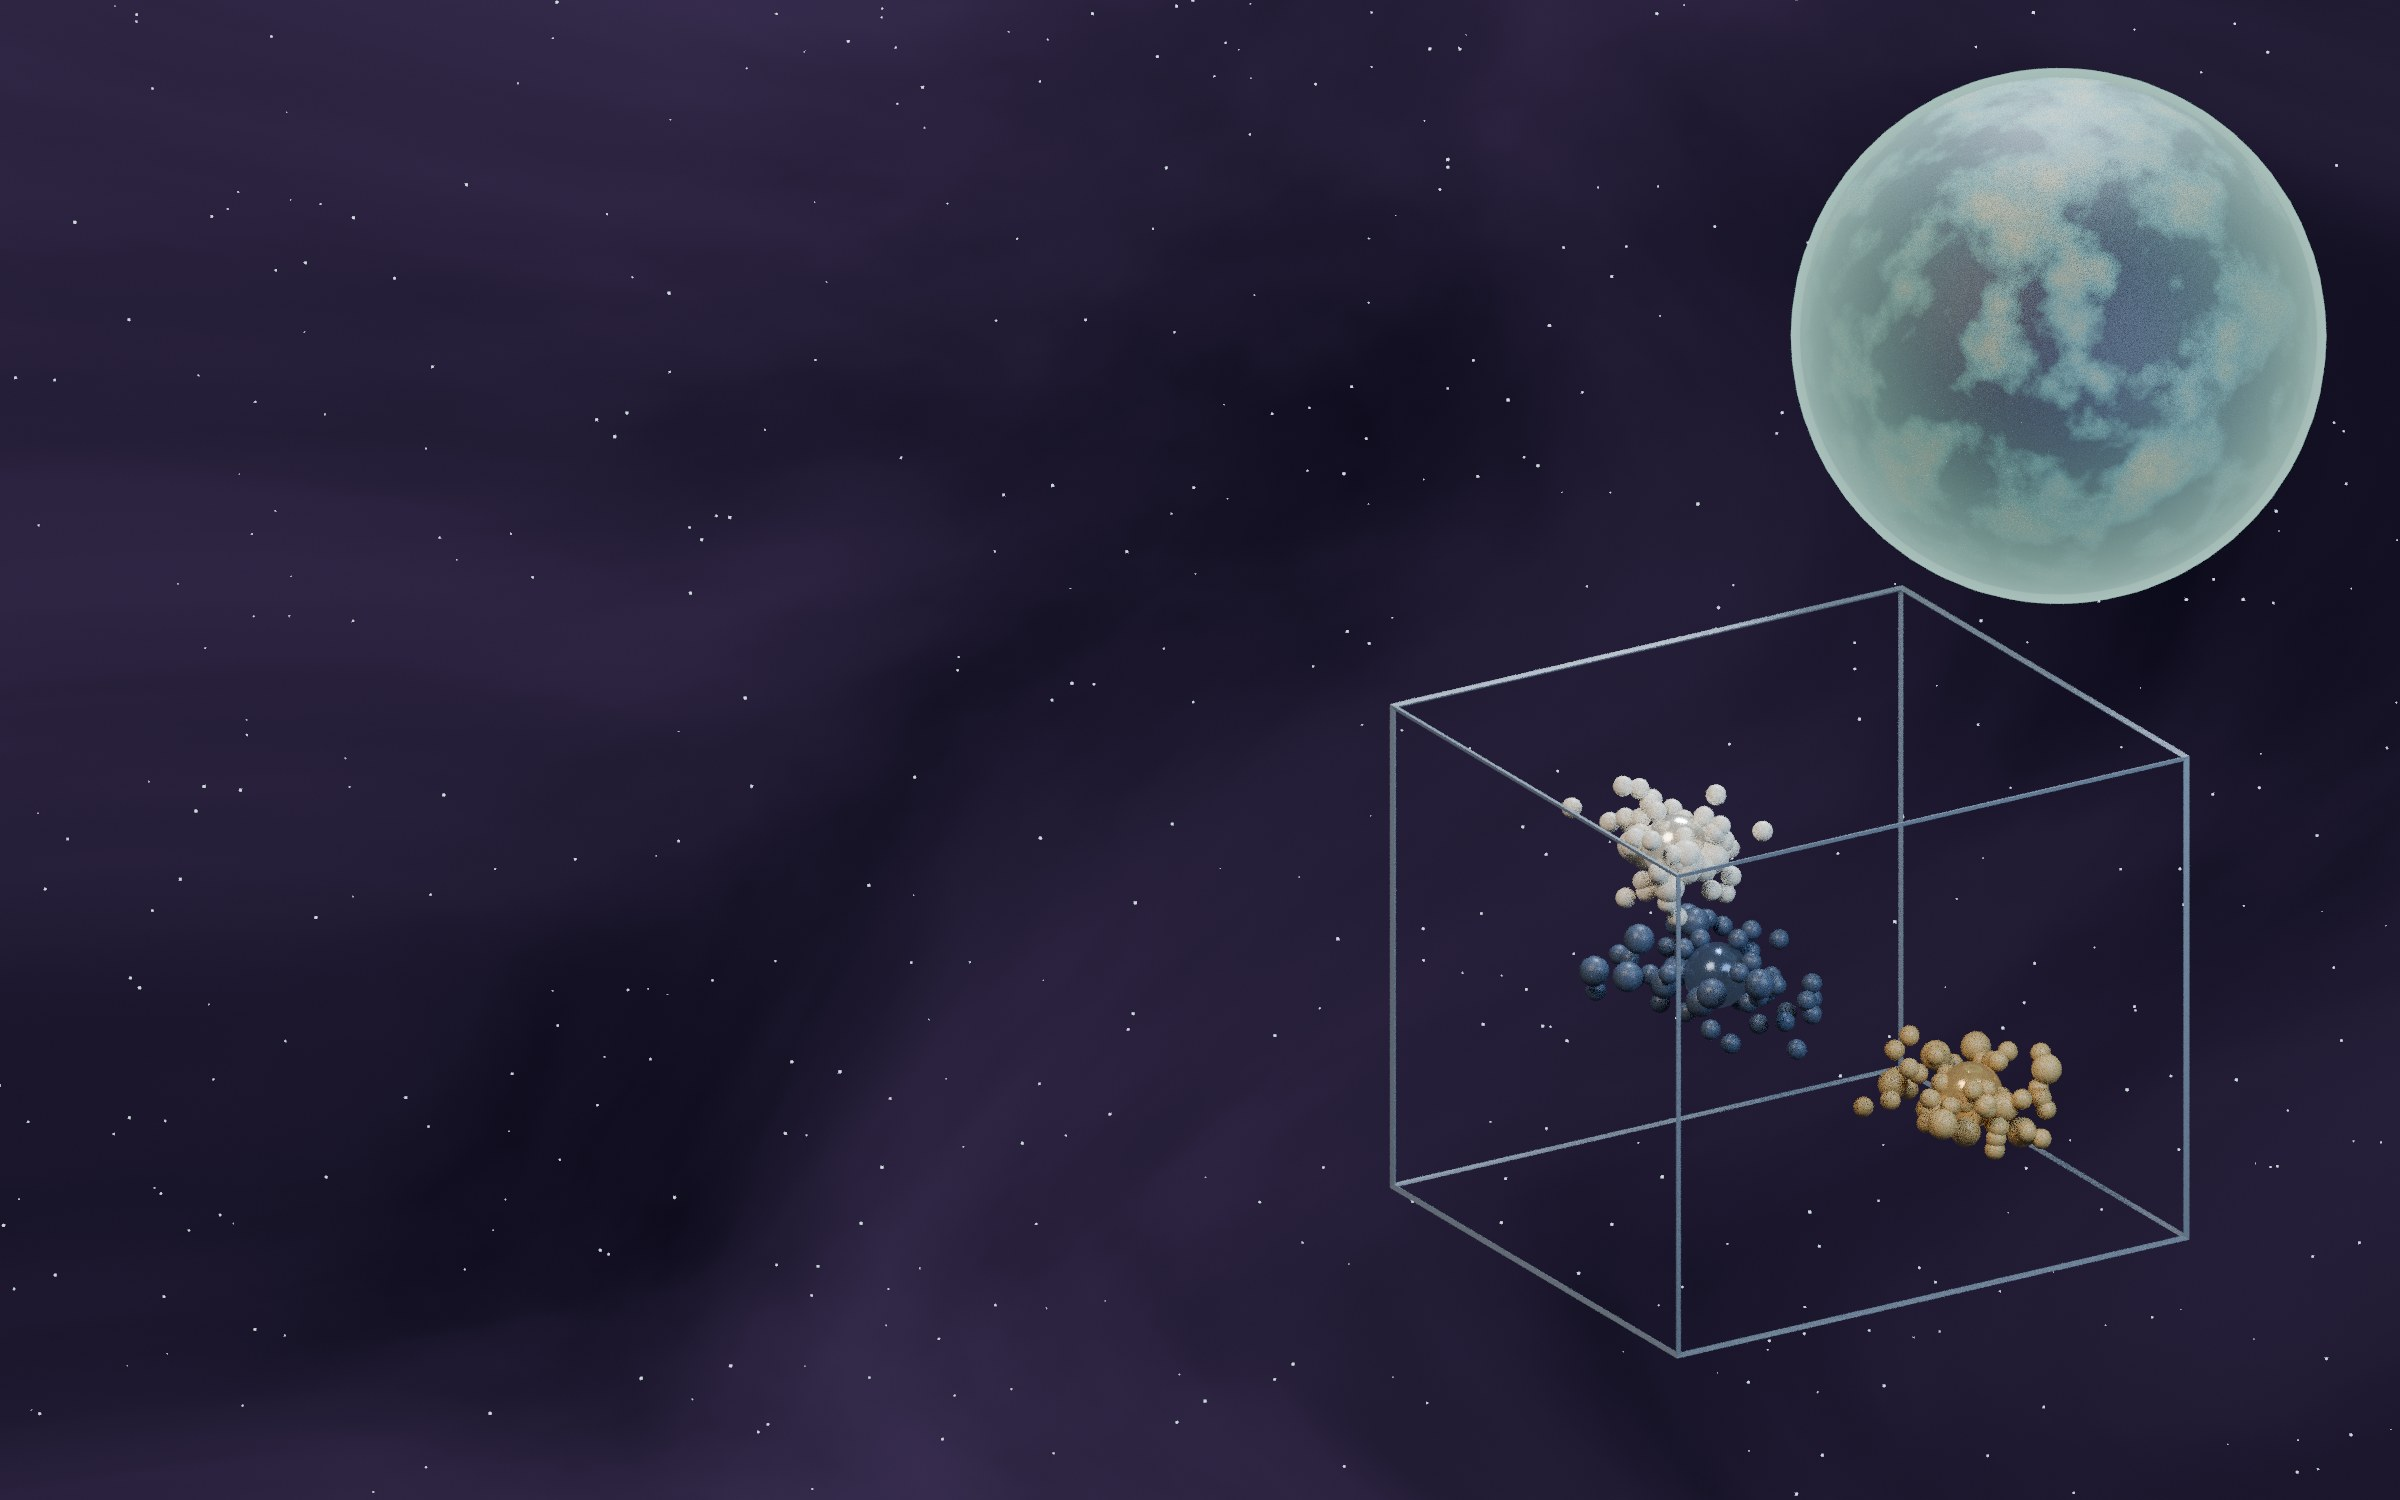
\includegraphics[width=20cm,height=12.5cm]{Scena/copertina.jpg}};}{}
\node[anchor=north west,inner sep=0] at([xshift=1.05cm,yshift=-1.10cm]current page.north west){\color{Mint}\bfseries\fontsize{23}{28}\selectfont SPEDIZIONE P11};
\node[anchor=north west,inner sep=0] at([xshift=1.07cm,yshift=-2.16cm]current page.north west){\color{white}\fontsize{9}{12}\selectfont MACROPROGETTO P11 · SCIENZE DELLA TERRA};
\draw[Mint,line width=1.5pt]([xshift=1.07cm,yshift=-2.78cm]current page.north west)--([xshift=2.6cm,yshift=-2.78cm]current page.north west);
\node[anchor=north west,inner sep=0] at([xshift=1.05cm,yshift=-3.35cm]current page.north west){\begin{minipage}{9.2cm}\raggedright\color{white}\bfseries\fontsize{28.5}{34.5}\selectfont Classificare\\nuove stazioni\\sintetiche\end{minipage}};
\node[anchor=north west,inner sep=0] at([xshift=1.07cm,yshift=-7.88cm]current page.north west){\begin{minipage}{8.9cm}\raggedright\color{Lilac}\fontsize{12.2}{17}\selectfont Diciotto stazioni, tre litologie\end{minipage}};
\node[anchor=north west,inner sep=0] at([xshift=1.07cm,yshift=-8.70cm]current page.north west){\begin{minipage}{8.9cm}\raggedright\color{white!75}\fontsize{10.3}{14.5}\selectfont Separazione dei dati, standardizzazione e classificatore dei centroidi\end{minipage}};
\node[anchor=north west,inner sep=0] at([xshift=1.07cm,yshift=-10.52cm]current page.north west){\color{white}\fontsize{10.5}{14}\selectfont GeoStat Lab · corso di Marzio De Corato};
\node[anchor=north west,inner sep=0] at([xshift=1.07cm,yshift=-11.17cm]current page.north west){\color{Mint}\fontsize{8.8}{11}\selectfont\href{https://creativecommons.org/licenses/by-nc-sa/4.0/}{Impaginazione da Tessera · CC BY-NC-SA 4.0}};
\end{tikzpicture}\end{frame}

\begin{frame}[plain]\hypertarget{slide2}{}
\bookmark[level=1,page=2]{Indice della presentazione}
\begin{tikzpicture}[remember picture,overlay]
\PilotChrome{Indice della presentazione}{PERCORSO}{2}{I titoli dell’indice aprono i capitoli. Il nome del capitolo in alto riporta a questa pagina.}
\node[anchor=north west,inner sep=0] at([xshift=.96cm,yshift=-2.12cm]current page.north west){\Colonna{9.40cm}{\PLabel{Capitoli}
{\fontsize{10.7}{13.5}\selectfont\hyperlink{slide4}{Bersaglio e protocollo di valutazione\hfill 4}\par}\vspace{.16cm}
{\fontsize{10.7}{13.5}\selectfont\hyperlink{slide8}{Geometria standardizzata e centroidi\hfill 8}\par}\vspace{.16cm}
{\fontsize{10.7}{13.5}\selectfont\hyperlink{slide13}{Prestazione e limiti dell’interpretazione\hfill 13}\par}\vspace{.16cm}
{\fontsize{10.7}{13.5}\selectfont\hyperlink{slide17}{Scheda del modello e consegna\hfill 17}\par}\vspace{.16cm}
{\fontsize{10.7}{13.5}\selectfont\hyperlink{slide19}{Laboratori della spedizione\hfill 19}\par}\vspace{.16cm}

}};
\node[anchor=north west,inner sep=0] at([xshift=10.85cm,yshift=-2.12cm]current page.north west){\Colonna{8.16cm}{\PLabel{Percorso di lettura}
\PBody{Il percorso fissa bersaglio e protocollo di valutazione, costruisce geometria standardizzata e centroidi, misura la prestazione sulle stazioni escluse e compila la scheda del modello. I laboratori finali riprendono le tre fasi della spedizione.}
\PInfo{Le pagine Scenario A e Confronto riprendono gli esperimenti nel browser con dati sintetici. I valori di partenza del simulatore differiscono da quelli del caso.}
\href{https://marzione00.github.io/Lab_Geo/\#modulo-P11}{\color{Classical}\bfseries Apri la spedizione P11 su GeoStat Lab}
}};
\end{tikzpicture}\end{frame}

\begin{frame}[plain]\hypertarget{slide3}{}
\bookmark[level=1,page=3]{Il classificatore dei centroidi riconosce la litologia di stazioni escluse dall’adattamento?}
\begin{tikzpicture}[remember picture,overlay]
\PilotChrome{{\fontsize{15.3}{19}\selectfont Il classificatore dei centroidi riconosce la litologia di stazioni escluse dall’adattamento?}}{IL CASO GUIDA}{3}{La copertina è una scena illustrativa: le sfere riproducono i provini in tre coordinate standardizzate, con i centroidi più grandi.}
\node[anchor=north west,inner sep=0] at([xshift=.96cm,yshift=-2.12cm]current page.north west){\Colonna{9.40cm}{{\centering\resizebox{0.97\linewidth}{!}{\begin{tikzpicture}[x=1cm,y=1cm,every node/.style={font=\sffamily\fontsize{10}{12}\selectfont,text=Ink}]
\draw[draw=Classical,fill=Classical!8,rounded corners=2mm,line width=.7pt] (0,0.00) rectangle (8.6,-0.78);
\node[circle,anchor=center,fill=Classical,inner sep=0,minimum size=.5cm,text=white,font=\sffamily\bfseries\fontsize{9}{10}\selectfont] at (.48,-0.39) {1};
\node[anchor=west,text width=7.4cm,align=left] at (.95,-0.39) {Bersaglio e protocollo di valutazione};
\draw[pEdge] (.48,-0.80)--(.48,-1.02);
\draw[draw=Classical,fill=Classical!8,rounded corners=2mm,line width=.7pt] (0,-1.04) rectangle (8.6,-1.82);
\node[circle,anchor=center,fill=Classical,inner sep=0,minimum size=.5cm,text=white,font=\sffamily\bfseries\fontsize{9}{10}\selectfont] at (.48,-1.43) {2};
\node[anchor=west,text width=7.4cm,align=left] at (.95,-1.43) {Geometria standardizzata e centroidi};
\draw[pEdge] (.48,-1.84)--(.48,-2.06);
\draw[draw=Classical,fill=Classical!8,rounded corners=2mm,line width=.7pt] (0,-2.08) rectangle (8.6,-2.86);
\node[circle,anchor=center,fill=Classical,inner sep=0,minimum size=.5cm,text=white,font=\sffamily\bfseries\fontsize{9}{10}\selectfont] at (.48,-2.47) {3};
\node[anchor=west,text width=7.4cm,align=left] at (.95,-2.47) {Prestazione e limiti dell’interpretazione};
\draw[pEdge] (.48,-2.88)--(.48,-3.10);
\draw[draw=Classical,fill=Classical!8,rounded corners=2mm,line width=.7pt] (0,-3.12) rectangle (8.6,-3.90);
\node[circle,anchor=center,fill=Classical,inner sep=0,minimum size=.5cm,text=white,font=\sffamily\bfseries\fontsize{9}{10}\selectfont] at (.48,-3.51) {4};
\node[anchor=west,text width=7.4cm,align=left] at (.95,-3.51) {Scheda del modello e consegna};
\draw[pEdge] (.48,-3.92)--(.48,-4.14);
\draw[draw=GeoB,fill=GeoB!8,rounded corners=2mm,line width=.7pt] (0,-4.16) rectangle (8.6,-4.94);
\node[circle,anchor=center,fill=GeoB,inner sep=0,minimum size=.5cm,text=white,font=\sffamily\bfseries\fontsize{9}{10}\selectfont] at (.48,-4.55) {L};
\node[anchor=west,text width=7.4cm,align=left] at (.95,-4.55) {Laboratori della spedizione};
\end{tikzpicture}
}\par}
\PSmall{Capitoli della spedizione; L indica i laboratori conclusivi.}
}};
\node[anchor=north west,inner sep=0] at([xshift=10.85cm,yshift=-2.12cm]current page.north west){\Colonna{8.16cm}{\PLabel{Il caso}
\PBody{Centottanta provini sintetici di diciotto stazioni, descritti da quattro ossidi e dalla densità, appartengono a tre litologie: Arenaria, Basalto e Calcare. La separazione segue le stazioni, per cui tre stazioni intere restano escluse dall’adattamento.}
\PInfo{Seguiremo il classificatore dalla standardizzazione appresa sul train ai centroidi, alla matrice di confusione e ai margini delle decisioni.}
}};
\end{tikzpicture}\end{frame}

\begin{frame}[plain]\hypertarget{slide4}{}
\bookmark[level=0,page=4]{Bersaglio e protocollo di valutazione}
\bookmark[level=1,page=4]{La classe viene prevista da cinque caratteristiche}
\begin{tikzpicture}[remember picture,overlay]
\PilotChrome{La classe viene prevista da cinque caratteristiche}{BERSAGLIO E PROTOCOLLO DI VALUTAZIONE}{4}{Il protocollo di valutazione deve corrispondere al tipo di nuova unità sulla quale si intende applicare il modello.}
\node[anchor=north west,inner sep=0] at([xshift=.96cm,yshift=-2.12cm]current page.north west){\Colonna{9.40cm}{{\centering\resizebox{0.90\linewidth}{!}{\begin{tikzpicture}[x=1cm,y=-.87cm,every node/.style={font=\fontsize{12.2}{15}\selectfont,text=Ink},arr/.style={-{Stealth[length=2mm]},line width=.8pt,draw=Classical}]\path[use as bounding box] (0,0) rectangle (7.45,6.2);
\draw[draw=Classical,fill=Classical!8,rounded corners=2pt,line width=.7pt] (0.6,0.7) rectangle (6.8,2.3);
\node[anchor=center,text=Ink,font=\fontsize{13}{15}\selectfont,text width=5.8cm,align=center] at (3.7,1.5) {$\mathrm{SiO}_2$, CaO, MgO, FeO e densità};
\draw[arr,draw=Classical] (3.7,2.6)--(3.7,3.3);
\draw[draw=Quantum,fill=Quantum!8,rounded corners=2pt,line width=.7pt] (1.2,3.6) rectangle (6.2,5.1);
\node[anchor=center,text=Ink,font=\fontsize{13}{15}\selectfont,text width=4.7cm,align=center] at (3.7,4.35) {Regola di classificazione};
\node[anchor=center,text=Ink,font=\fontsize{11.5}{15}\selectfont,text width=6.8cm,align=center] at (3.7,6) {Tre classi note del generatore sintetico.};

\end{tikzpicture}}\par}
}};
\node[anchor=north west,inner sep=0] at([xshift=10.85cm,yshift=-2.12cm]current page.north west){\Colonna{8.16cm}{\PBody{Il progetto assegna ciascun campione a una delle tre litologie sintetiche, Arenaria, Basalto e Calcare, utilizzando quattro composizioni in ossidi e la densità. Il campione comprende centottanta provini raccolti in diciotto stazioni simulate. La domanda riguarda il trasferimento a stazioni escluse dall’adattamento, per cui la separazione avviene per stazioni intere e lascia insieme i provini di ciascuna. Il caso riutilizza dati già incontrati nel percorso didattico e applica una procedura prefissata; il risultato non costituisce una valutazione finale inedita di un modello scelto dopo ripetuti confronti.}
}};
\end{tikzpicture}\end{frame}

\begin{frame}[plain]\hypertarget{slide5}{}
\bookmark[level=1,page=5]{La stazione resta interamente in un insieme}
\begin{tikzpicture}[remember picture,overlay]
\PilotChrome{La stazione resta interamente in un insieme}{BERSAGLIO E PROTOCOLLO DI VALUTAZIONE}{5}{La separazione per gruppi conserva il livello al quale si vuole valutare la generalizzazione.}
\node[anchor=north west,inner sep=0] at([xshift=.96cm,yshift=-2.12cm]current page.north west){\Colonna{9.40cm}{{\centering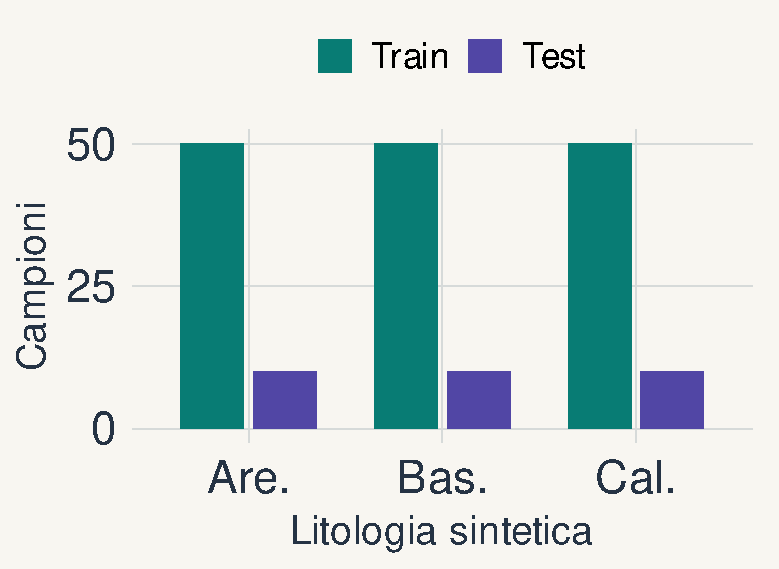
\includegraphics[width=\linewidth,height=6.15cm,keepaspectratio]{Figure/F01.pdf}\par}
\PSmall{$\mathcal S$: insieme delle stazioni, distinto fra train e test. Are.: Arenaria; Bas.: Basalto; Cal.: Calcare.}
}};
\node[anchor=north west,inner sep=0] at([xshift=10.85cm,yshift=-2.12cm]current page.north west){\Colonna{8.16cm}{\PBody{Quindici stazioni, con centocinquanta campioni, appartengono all’adattamento; le tre restanti, con trenta campioni, costituiscono il test. Nessuna stazione compare in entrambi gli insiemi. La divisione conserva dieci provini per stazione e, nel test, una stazione per ciascuna classe. Il controllo dell’intersezione degli identificativi territoriali verifica quindi una condizione più forte della semplice assenza di righe duplicate, evitando che provini dello stesso gruppo forniscano informazione sia alla costruzione sia alla valutazione della regola.}
\par\smallskip{\centering\adjustbox{max width=.98\linewidth}{$\displaystyle \mathcal S_{train}\cap\mathcal S_{test}=\varnothing$}\par\smallskip}
}};
\end{tikzpicture}\end{frame}

\begin{frame}[plain]\hypertarget{slide6}{}
\bookmark[level=1,page=6]{Il controllo conserva la struttura della divisione}
\begin{tikzpicture}[remember picture,overlay]
\PilotChrome{Il controllo conserva la struttura della divisione}{BERSAGLIO E PROTOCOLLO DI VALUTAZIONE}{6}{La divisione deve precedere ogni trasformazione che apprende parametri dai dati.}
\node[anchor=north west,inner sep=0] at([xshift=.96cm,yshift=-2.12cm]current page.north west){\Colonna{9.40cm}{\PBody{Il frammento ricostruisce i due insiemi dalla variabile di appartenenza già presente nei dati e ne verifica numerosità e disgiunzione delle stazioni. La tabella per litologia rende esplicito anche il bilanciamento delle classi. Il controllo precede standardizzazione e calcolo dei centroidi, affinché nessuna statistica della risposta o dei predittori del test entri nella costruzione della regola. Le etichette del test verranno utilizzate soltanto dopo aver prodotto le classificazioni con il procedimento definito.}
}};
\node[anchor=north west,inner sep=0] at([xshift=10.85cm,yshift=-2.12cm]current page.north west){\Colonna{8.16cm}{\begin{tcolorbox}[enhanced,arc=1.7mm,boxrule=.6pt,colback=white,colframe=Classical!60!Navy,colbacktitle=Navy,coltitle=white,fonttitle=\bfseries\small,title={R · calcolo riproducibile},left=1.7mm,right=1.3mm,top=1.1mm,bottom=1.1mm,before skip=1mm,after skip=1.0mm]\lstinputlisting[style=GeoR,language=R,basicstyle=\ttfamily\fontsize{8.6}{11.4}\selectfont]{Codice/separazione.R}\end{tcolorbox}
\PLabel{Risultato in R}
\begin{tcolorbox}[colback=GeoTint,colframe=Rule,boxrule=.5pt,arc=1.4mm,left=2mm,right=1mm,top=1mm,bottom=1mm]{\fontsize{8.4}{10.9}\selectfont\ttfamily \mbox{\ \ \ \ \ \ \ \ \ \ }\\\mbox{\ \ \ \ \ \ \ \ \ \ \ test\ train}\\\mbox{\ \ Arenaria\ \ \ 10\ \ \ \ 50}\\\mbox{\ \ Basalto\ \ \ \ 10\ \ \ \ 50}\\\mbox{\ \ Calcare\ \ \ \ 10\ \ \ \ 50}}\end{tcolorbox}
}};
\end{tikzpicture}\end{frame}

\begin{frame}[plain]\hypertarget{slide7}{}
\bookmark[level=1,page=7]{Il riferimento risolve un pareggio dichiarato}
\begin{tikzpicture}[remember picture,overlay]
\PilotChrome{Il riferimento risolve un pareggio dichiarato}{BERSAGLIO E PROTOCOLLO DI VALUTAZIONE}{7}{Anche la procedura di riferimento deve essere definita usando esclusivamente l’insieme di adattamento.}
\node[anchor=north west,inner sep=0] at([xshift=.96cm,yshift=-2.12cm]current page.north west){\Colonna{9.40cm}{{\centering\resizebox{0.90\linewidth}{!}{\begin{tikzpicture}[x=1cm,y=-.87cm,every node/.style={font=\fontsize{12.2}{15}\selectfont,text=Ink},arr/.style={-{Stealth[length=2mm]},line width=.8pt,draw=Classical}]\path[use as bounding box] (0,0) rectangle (7.45,6.2);
\draw[draw=Classical,fill=Classical!8,rounded corners=2pt,line width=.7pt] (0.6,0.7) rectangle (6.8,2);
\node[anchor=center,text=Ink,font=\fontsize{12}{15}\selectfont,text width=6cm,align=center] at (3.7,1.35) {50 Arenaria, 50 Basalto, 50 Calcare};
\draw[arr,draw=Classical] (3.7,2.3)--(3.7,3);
\draw[draw=Quantum,fill=Quantum!8,rounded corners=2pt,line width=.7pt] (0.6,3.3) rectangle (6.8,4.6);
\node[anchor=center,text=Ink,font=\fontsize{12}{15}\selectfont,text width=6cm,align=center] at (3.7,3.95) {Pareggio: ordine alfabetico};
\node[anchor=center,text=Ink,font=\fontsize{13}{15}\selectfont,text width=6.8cm,align=center] at (3.7,5.7) {Previsione costante: Arenaria.};

\end{tikzpicture}}\par}
\PSmall{$n_{c,train}$: campioni train della classe c; $\widehat c_0$: classe assegnata. $Acc_0$: quota corretta nel test. Il pareggio segue l’ordine alfabetico.}
}};
\node[anchor=north west,inner sep=0] at([xshift=10.85cm,yshift=-2.12cm]current page.north west){\Colonna{8.16cm}{\PBody{La procedura elementare assegna a tutti i nuovi campioni la classe più frequente nell’adattamento. Poiché le tre classi hanno cinquanta osservazioni ciascuna, il pareggio viene risolto secondo l’ordine alfabetico e la previsione costante diventa Arenaria. Nel test bilanciato questa regola classifica correttamente dieci campioni su trenta, con accuratezza pari a un terzo. Il riferimento quantifica così la prestazione ottenibile senza usare le caratteristiche e rende interpretabile il contributo del classificatore successivo.}
\par\smallskip{\centering\adjustbox{max width=.98\linewidth}{$\displaystyle \widehat c_0=\arg\max_c n_{c,train},\qquad Acc_0=\frac{10}{30}$}\par\smallskip}
}};
\end{tikzpicture}\end{frame}

\begin{frame}[plain]\hypertarget{slide8}{}
\bookmark[level=0,page=8]{Geometria standardizzata e centroidi}
\bookmark[level=1,page=8]{La standardizzazione apprende soltanto dal train}
\begin{tikzpicture}[remember picture,overlay]
\PilotChrome{La standardizzazione apprende soltanto dal train}{GEOMETRIA STANDARDIZZATA E CENTROIDI}{8}{I parametri della trasformazione fanno parte del modello appreso e devono essere conservati insieme al classificatore.}
\node[anchor=north west,inner sep=0] at([xshift=.96cm,yshift=-2.12cm]current page.north west){\Colonna{9.40cm}{\PBody{Le composizioni e la densità hanno scale numeriche differenti, che influenzerebbero direttamente una distanza euclidea. Ogni variabile viene quindi centrata sulla propria media nell’adattamento e divisa per la deviazione standard dello stesso insieme, calcolata con denominatore n meno uno. Questi parametri vengono conservati e applicati senza ricalcolo ai trenta campioni di test. La trasformazione stabilisce la metrica del classificatore; includere il test nel calcolo delle scale introdurrebbe informazione del campione di verifica nella procedura da valutare.}
\par\smallskip{\centering\adjustbox{max width=.98\linewidth}{$\displaystyle z_{ij}=\frac{x_{ij}-\overline x_{j,train}}{s_{j,train}}$}\par\smallskip}
}};
\node[anchor=north west,inner sep=0] at([xshift=10.85cm,yshift=-2.12cm]current page.north west){\Colonna{8.16cm}{\PInfo{i: campione; j: una delle cinque variabili; $x_{ij}$: valore originario; $z_{ij}$: valore standardizzato. $\overline x_{j,train}$ e $s_{j,train}$ sono media e deviazione standard nei 150 campioni train, con denominatore 149 per la varianza. Le medie standardizzate sono nulle e le deviazioni unitarie entro la tolleranza numerica; tali proprietà non sono richieste nel test.}
}};
\end{tikzpicture}\end{frame}

\begin{frame}[plain]\hypertarget{slide9}{}
\bookmark[level=1,page=9]{Il centroide rappresenta la media di una classe}
\begin{tikzpicture}[remember picture,overlay]
\PilotChrome{Il centroide rappresenta la media di una classe}{GEOMETRIA STANDARDIZZATA E CENTROIDI}{9}{La geometria del centroide riassume la posizione media, senza modellare l’intera distribuzione della classe.}
\node[anchor=north west,inner sep=0] at([xshift=.96cm,yshift=-2.12cm]current page.north west){\Colonna{9.40cm}{\PBody{Per ciascuna litologia si calcola il vettore medio delle cinque caratteristiche standardizzate nei soli campioni di adattamento. La carta cromatica mostra i tre centroidi, consentendo di riconoscere quali variabili caratterizzino la posizione media dei gruppi nel generatore sintetico. Il colore esprime deviazioni standard rispetto alla media complessiva del train. Un centroide riassume la posizione della classe e lascia esclusa la sua dispersione interna, che potrebbe diventare rilevante quando gruppi differenti mostrano forme o varianze molto diverse.}
\par\smallskip{\centering\adjustbox{max width=.98\linewidth}{$\displaystyle \mathbf c_k=\frac1{n_{k,train}}\sum_{i\in train:Y_i=k}\mathbf z_i$}\par\smallskip}
}};
\node[anchor=north west,inner sep=0] at([xshift=10.85cm,yshift=-2.12cm]current page.north west){\Colonna{8.16cm}{{\centering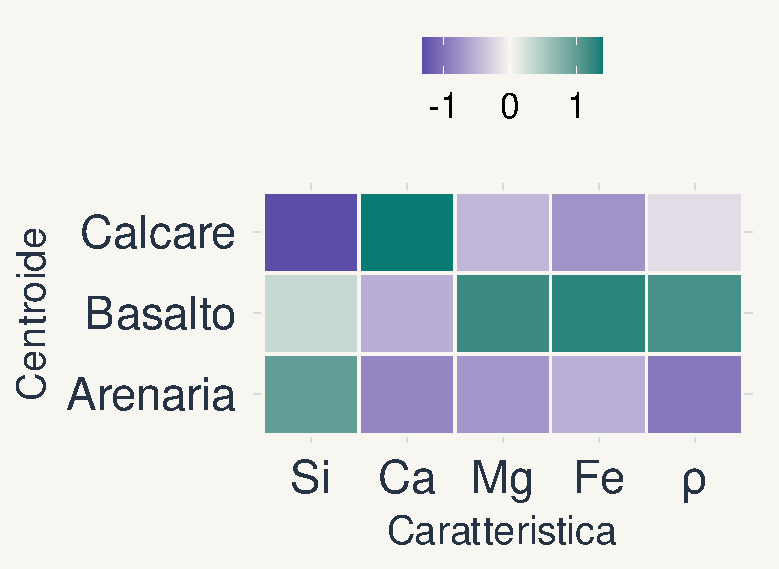
\includegraphics[width=\linewidth,height=5.3cm,keepaspectratio]{Figure/F03.pdf}\par}
\PSmall{$Y_i$: classe di i; $n_{k,train}$: numerosità della classe k; $\mathbf z_i$: vettore standardizzato; $\mathbf c_k$: sua media. Si, Ca, Mg, Fe: ossidi; $\rho$: densità.}
}};
\end{tikzpicture}\end{frame}

\begin{frame}[plain]\hypertarget{slide10}{}
\bookmark[level=1,page=10]{La regola minimizza una distanza quadratica}
\begin{tikzpicture}[remember picture,overlay]
\PilotChrome{La regola minimizza una distanza quadratica}{GEOMETRIA STANDARDIZZATA E CENTROIDI}{10}{La regola di classificazione è definita nello spazio trasformato, la cui metrica dipende dalle scale apprese.}
\node[anchor=north west,inner sep=0] at([xshift=.96cm,yshift=-2.12cm]current page.north west){\Colonna{9.40cm}{{\centering\resizebox{0.90\linewidth}{!}{\begin{tikzpicture}[x=1cm,y=-.87cm,every node/.style={font=\fontsize{12.2}{15}\selectfont,text=Ink},arr/.style={-{Stealth[length=2mm]},line width=.8pt,draw=Classical}]\path[use as bounding box] (0,0) rectangle (7.45,6.2);
\draw[Rule,line width=.8pt] (0.7,5.3)--(6.7,5.3);
\draw[Rule,line width=.8pt] (0.7,5.3)--(0.7,0.7);
\node[anchor=center,text=Classical,font=\fontsize{15}{15}\selectfont] at (2.1,2) {$\mathbf c_A$};
\node[anchor=center,text=Quantum,font=\fontsize{15}{15}\selectfont] at (5.4,3.8) {$\mathbf c_B$};
\node[anchor=center,text=Ink,font=\fontsize{16}{15}\selectfont] at (3.6,2.7) {$\mathbf z$};
\draw[Classical,line width=.8pt] (2.4,2.15)--(3.3,2.55);
\draw[Quantum,line width=.8pt] (3.9,2.9)--(5,3.6);
\node[anchor=center,text=Ink,font=\fontsize{10.8}{15}\selectfont,text width=6.8cm,align=center] at (3.7,6) {Schema in due dimensioni; calcolo effettivo in cinque.};

\end{tikzpicture}}\par}
\PSmall{$z_j$: caratteristica standardizzata j; $c_{kj}$: coordinata j del centroide k; $\widehat y$: classe assegnata. Si confrontano cinque coordinate e tre classi.}
}};
\node[anchor=north west,inner sep=0] at([xshift=10.85cm,yshift=-2.12cm]current page.north west){\Colonna{8.16cm}{\PBody{Un nuovo vettore standardizzato viene assegnato al centroide più vicino nella metrica euclidea a cinque dimensioni. Poiché la radice quadrata conserva l’ordine, il codice confronta direttamente le somme dei quadrati degli scarti. L’eventuale pareggio segue l’ordine alfabetico dichiarato delle classi. La decisione dipende quindi da scale, centroidi e convenzione di assegnazione, che devono essere tutti disponibili per riprodurre la previsione su un nuovo campione.}
\par\smallskip{\centering\adjustbox{max width=.98\linewidth}{$\displaystyle \widehat y(\mathbf z)=\arg\min_k\sum_{j=1}^{5}(z_j-c_{kj})^2$}\par\smallskip}
}};
\end{tikzpicture}\end{frame}

\begin{frame}[plain]\hypertarget{slide11}{}
\bookmark[level=1,page=11]{Il confine fra due centroidi è un iperpiano}
\begin{tikzpicture}[remember picture,overlay]
\PilotChrome{Il confine fra due centroidi è un iperpiano}{GEOMETRIA STANDARDIZZATA E CENTROIDI}{11}{La forma del confine deriva dalla regola matematica di distanza e non deve essere dedotta soltanto da una proiezione grafica.}
\node[anchor=north west,inner sep=0] at([xshift=.96cm,yshift=-2.12cm]current page.north west){\Colonna{9.40cm}{\PBody{Le osservazioni equidistanti da due centroidi soddisfano l’uguaglianza fra le due distanze quadratiche. Espandendo i quadrati, il termine comune nella norma dell’osservazione si elimina e rimane un’equazione lineare nel vettore standardizzato. Il confine è quindi un iperpiano, che diventa una retta in una rappresentazione bidimensionale. Con tre classi, ciascuna regione è determinata dal confronto simultaneo con gli altri centroidi; la struttura risultante dipende dalla metrica scelta e dalle posizioni delle medie di classe.}
\par\smallskip{\centering\adjustbox{max width=.98\linewidth}{$\displaystyle 2\mathbf z^T(\mathbf c_b-\mathbf c_a)=\|\mathbf c_b\|^2-\|\mathbf c_a\|^2$}\par\smallskip}
}};
\node[anchor=north west,inner sep=0] at([xshift=10.85cm,yshift=-2.12cm]current page.north west){\Colonna{8.16cm}{\PInfo{$\mathbf z\in\mathbb R^5$: osservazione standardizzata; $\mathbf c_a,\mathbf c_b$: centroidi di due classi. T indica la trasposta e $\|\mathbf v\|^2=\sum_{j=1}^5v_j^2$ la norma euclidea al quadrato. Se i centroidi sono distinti, l’equazione definisce un iperpiano. Trasformare le scale può modificare il confine nelle variabili originarie.}
}};
\end{tikzpicture}\end{frame}

\begin{frame}[plain]\hypertarget{slide12}{}
\bookmark[level=1,page=12]{La proiezione conserva soltanto due coordinate}
\begin{tikzpicture}[remember picture,overlay]
\PilotChrome{La proiezione conserva soltanto due coordinate}{GEOMETRIA STANDARDIZZATA E CENTROIDI}{12}{Una proiezione grafica illustra la geometria senza sostituire il calcolo nello spazio completo dei predittori.}
\node[anchor=north west,inner sep=0] at([xshift=.96cm,yshift=-2.12cm]current page.north west){\Colonna{9.40cm}{{\centering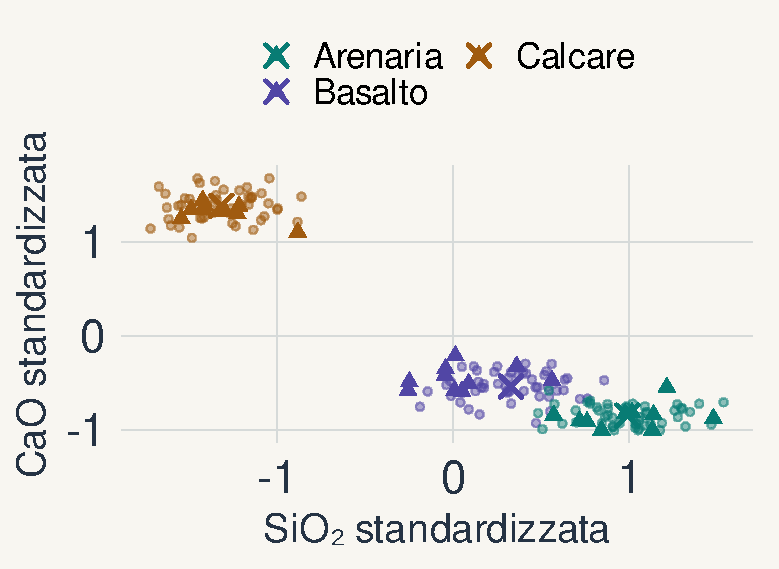
\includegraphics[width=\linewidth,height=6.15cm,keepaspectratio]{Figure/F02.pdf}\par}
\PSmall{Proiezione SiO$_2$–CaO: train, test e centroidi; decisione in cinque dimensioni.}
}};
\node[anchor=north west,inner sep=0] at([xshift=10.85cm,yshift=-2.12cm]current page.north west){\Colonna{8.16cm}{\PBody{Il diagramma rappresenta silice e ossido di calcio standardizzati, con punti per il train, triangoli per il test e croci per i centroidi. La separazione visibile aiuta a comprendere la struttura del campione sintetico, ma il classificatore utilizza anche magnesio, ferro e densità. La figura è dunque una proiezione del problema e non rappresenta tutte le distanze né i confini effettivi della decisione. Una sovrapposizione in questa vista potrebbe scomparire nello spazio completo, mentre una separazione apparente richiede comunque verifica numerica.}
}};
\end{tikzpicture}\end{frame}

\begin{frame}[plain]\hypertarget{slide13}{}
\bookmark[level=0,page=13]{Prestazione e limiti dell’interpretazione}
\bookmark[level=1,page=13]{Il modello conservato ricostruisce le decisioni}
\begin{tikzpicture}[remember picture,overlay]
\PilotChrome{Il modello conservato ricostruisce le decisioni}{PRESTAZIONE E LIMITI DELL’INTERPRETAZIONE}{13}{Riprodurre una decisione richiede l’intera trasformazione e l’ordine delle caratteristiche, oltre ai soli centroidi.}
\node[anchor=north west,inner sep=0] at([xshift=.96cm,yshift=-2.12cm]current page.north west){\Colonna{9.40cm}{\PBody{Il file del modello contiene nomi e ordine delle variabili, medie, scale, centroidi e classi. Il frammento rilegge questi oggetti e calcola le previsioni senza stimare nuovi parametri, rendendo esplicito il passaggio dall’adattamento all’applicazione. Le classi osservate entrano soltanto nella tabella finale di confronto. La rilettura viene verificata rispetto all’oggetto salvato, poiché una ricostruzione parziale che omettesse l’ordine delle colonne potrebbe produrre distanze errate anche usando gli stessi valori numerici.}
}};
\node[anchor=north west,inner sep=0] at([xshift=10.85cm,yshift=-2.12cm]current page.north west){\Colonna{8.16cm}{\begin{tcolorbox}[enhanced,arc=1.7mm,boxrule=.6pt,colback=white,colframe=Classical!60!Navy,colbacktitle=Navy,coltitle=white,fonttitle=\bfseries\small,title={R · calcolo riproducibile},left=1.7mm,right=1.3mm,top=1.1mm,bottom=1.1mm,before skip=1mm,after skip=1.0mm]\lstinputlisting[style=GeoR,language=R,basicstyle=\ttfamily\fontsize{8.6}{11.4}\selectfont]{Codice/previsione.R}\end{tcolorbox}
\PLabel{Risultato in R}
\begin{tcolorbox}[colback=GeoTint,colframe=Rule,boxrule=.5pt,arc=1.4mm,left=2mm,right=1mm,top=1mm,bottom=1mm]{\fontsize{8.4}{10.9}\selectfont\ttfamily \mbox{corretta}\\\mbox{TRUE\ }\\\mbox{\ \ 30\ }}\end{tcolorbox}
}};
\end{tikzpicture}\end{frame}

\begin{frame}[plain]\hypertarget{slide14}{}
\bookmark[level=1,page=14]{La matrice di confusione conserva i conteggi}
\begin{tikzpicture}[remember picture,overlay]
\PilotChrome{La matrice di confusione conserva i conteggi}{PRESTAZIONE E LIMITI DELL’INTERPRETAZIONE}{14}{Un’accuratezza perfetta nel campione disponibile non dimostra assenza di errore nella popolazione di applicazione.}
\node[anchor=north west,inner sep=0] at([xshift=.96cm,yshift=-2.12cm]current page.north west){\Colonna{9.40cm}{{\centering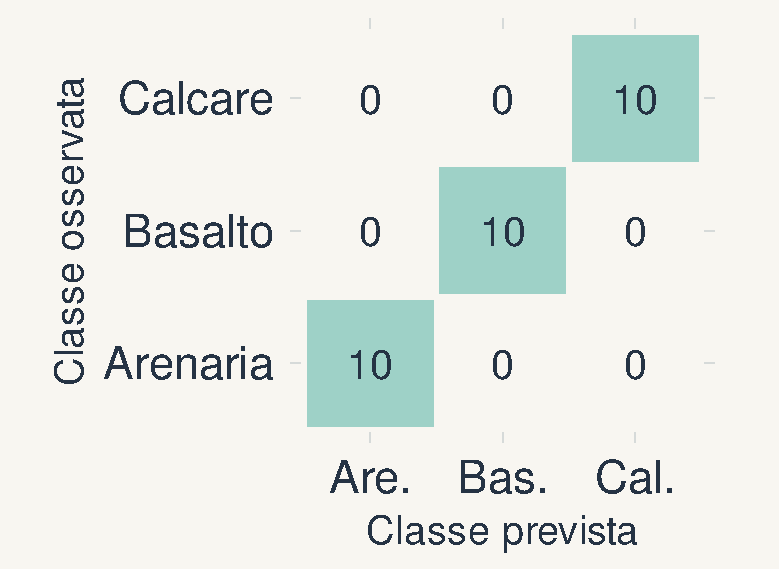
\includegraphics[width=\linewidth,height=6.15cm,keepaspectratio]{Figure/F04.pdf}\par}
\PSmall{$y_i$: classe osservata; $\widehat y_i$: prevista; $\mathbf1$: vale 1 se coincidono, 0 altrimenti. Are.: Arenaria; Bas.: Basalto; Cal.: Calcare.}
}};
\node[anchor=north west,inner sep=0] at([xshift=10.85cm,yshift=-2.12cm]current page.north west){\Colonna{8.16cm}{\PBody{Tutti i trenta campioni di test vengono assegnati alla classe osservata, con dieci casi sulla diagonale per ciascuna litologia. L’accuratezza risulta quindi pari a uno in questo campione. La matrice conserva i denominatori e rende controllabile l’assenza di errori fra coppie di classi, senza trasformare l’esito in una garanzia universale. I trenta provini provengono soltanto da tre stazioni e dallo stesso generatore sintetico, condizioni che limitano l’interpretazione rispetto a un’applicazione su rocce reali.}
\par\smallskip{\centering\adjustbox{max width=.98\linewidth}{$\displaystyle Acc=\frac1{30}\sum_{i\in test}\mathbf1\{\widehat y_i=y_i\}=1$}\par\smallskip}
}};
\end{tikzpicture}\end{frame}

\begin{frame}[plain]\hypertarget{slide15}{}
\bookmark[level=1,page=15]{Il confronto quantifica il contributo delle variabili}
\begin{tikzpicture}[remember picture,overlay]
\PilotChrome{{\fontsize{15.3}{19}\selectfont Il confronto quantifica il contributo delle variabili}}{PRESTAZIONE E LIMITI DELL’INTERPRETAZIONE}{15}{La prestazione viene attribuita alla procedura e alla distribuzione effettivamente valutate.}
\node[anchor=north west,inner sep=0] at([xshift=.96cm,yshift=-2.12cm]current page.north west){\Colonna{9.40cm}{{\centering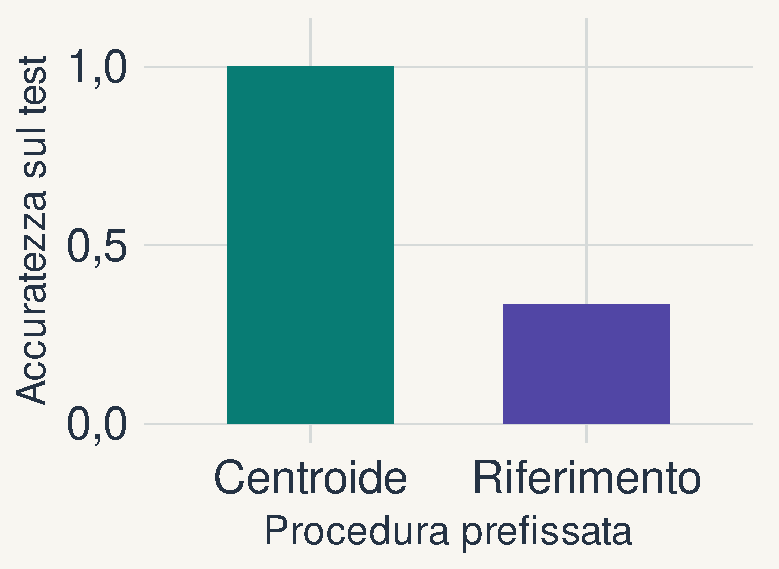
\includegraphics[width=\linewidth,height=6.15cm,keepaspectratio]{Figure/F05.pdf}\par}
\PSmall{Accuratezze sullo stesso test: riferimento costante e centroidi.}
}};
\node[anchor=north west,inner sep=0] at([xshift=10.85cm,yshift=-2.12cm]current page.north west){\Colonna{8.16cm}{\PBody{L’accuratezza passa da un terzo per la previsione costante a uno per il classificatore dei centroidi. Entrambe le procedure sono valutate sugli stessi trenta campioni, così che il confronto conservi il medesimo denominatore. Il guadagno è coerente con la separazione costruita nel generatore sintetico e dimostra il funzionamento del procedimento didattico. L’impiego su nuove stazioni reali richiederebbe dati indipendenti, verifiche delle unità e valutazione delle differenze fra distribuzione di adattamento e contesto operativo.}
}};
\end{tikzpicture}\end{frame}

\begin{frame}[plain]\hypertarget{slide16}{}
\bookmark[level=1,page=16]{Il margine misura una separazione geometrica}
\begin{tikzpicture}[remember picture,overlay]
\PilotChrome{Il margine misura una separazione geometrica}{PRESTAZIONE E LIMITI DELL’INTERPRETAZIONE}{16}{La distanza dal concorrente misura una proprietà geometrica; la probabilità di errore richiede una valutazione ulteriore.}
\node[anchor=north west,inner sep=0] at([xshift=.96cm,yshift=-2.12cm]current page.north west){\Colonna{9.40cm}{{\centering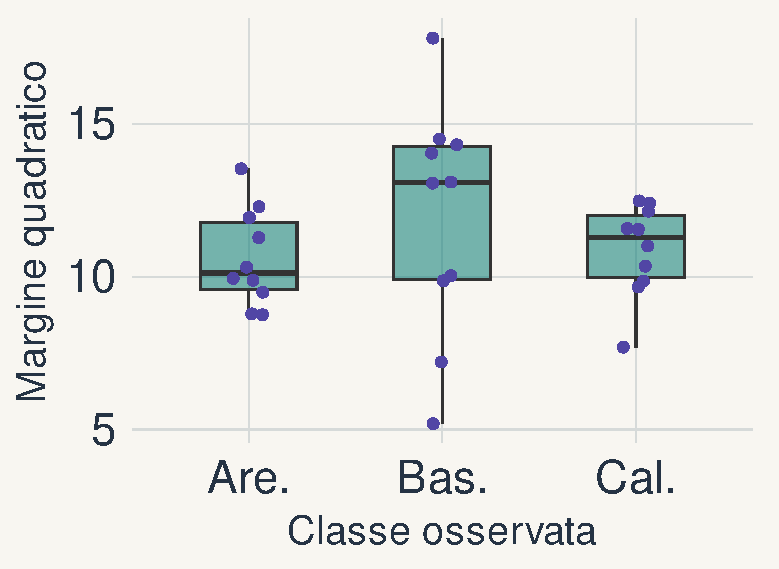
\includegraphics[width=\linewidth,height=6.15cm,keepaspectratio]{Figure/F06.pdf}\par}
\PSmall{$d^2_{i,(1)},d^2_{i,(2)}$: prima e seconda distanza quadratica in ordine crescente. $\Delta_i$: margine per il campione i, adimensionale.}
}};
\node[anchor=north west,inner sep=0] at([xshift=10.85cm,yshift=-2.12cm]current page.north west){\Colonna{8.16cm}{\PBody{La differenza fra la seconda distanza quadratica più piccola e la prima misura quanto la decisione sia separata dalla classe concorrente più vicina. Nel campione tutti i margini sono positivi, coerentemente con assegnazioni senza pareggio. La distribuzione per classe descrive la geometria del classificatore e può aiutare a individuare decisioni più prossime al confine. Il margine non è una probabilità calibrata di correttezza e potrebbe essere ampio anche per un campione esterno al dominio rappresentato dalle tre classi note.}
\par\smallskip{\centering\adjustbox{max width=.98\linewidth}{$\displaystyle \Delta_i=d^2_{i,(2)}-d^2_{i,(1)}$}\par\smallskip}
}};
\end{tikzpicture}\end{frame}

\begin{frame}[plain]\hypertarget{slide17}{}
\bookmark[level=0,page=17]{Scheda del modello e consegna}
\bookmark[level=1,page=17]{La scheda conserva dominio e condizioni d’uso}
\begin{tikzpicture}[remember picture,overlay]
\PilotChrome{La scheda conserva dominio e condizioni d’uso}{SCHEDA DEL MODELLO E CONSEGNA}{17}{Il modello conservato deve essere accompagnato dalle condizioni entro le quali la sua prestazione è stata osservata.}
\node[anchor=north west,inner sep=0] at([xshift=.96cm,yshift=-2.12cm]current page.north west){\Colonna{9.40cm}{{\centering\resizebox{0.90\linewidth}{!}{\begin{tikzpicture}[x=1cm,y=-.87cm,every node/.style={font=\fontsize{12.2}{15}\selectfont,text=Ink},arr/.style={-{Stealth[length=2mm]},line width=.8pt,draw=Classical}]\path[use as bounding box] (0,0) rectangle (7.45,6.2);
\draw[draw=Classical,fill=Classical!8,rounded corners=2pt,line width=.7pt] (0.6,0.6) rectangle (6.8,2);
\node[anchor=center,text=Ink,font=\fontsize{12}{15}\selectfont,text width=5.8cm,align=center] at (3.7,1.3) {Variabili, unità e trasformazione};
\draw[draw=Quantum,fill=Quantum!8,rounded corners=2pt,line width=.7pt] (0.6,2.5) rectangle (6.8,3.9);
\node[anchor=center,text=Ink,font=\fontsize{12}{15}\selectfont,text width=5.8cm,align=center] at (3.7,3.2) {Dati di valutazione e prestazione};
\draw[draw=Classical,fill=Classical!8,rounded corners=2pt,line width=.7pt] (0.6,4.4) rectangle (6.8,5.8);
\node[anchor=center,text=Ink,font=\fontsize{12}{15}\selectfont,text width=5.8cm,align=center] at (3.7,5.1) {Dominio, limiti e versioni};

\end{tikzpicture}}\par}
}};
\node[anchor=north west,inner sep=0] at([xshift=10.85cm,yshift=-2.12cm]current page.north west){\Colonna{8.16cm}{\PBody{La scheda del modello registra bersaglio, origine sintetica, variabili e unità, numerosità per insieme, regola di standardizzazione, metrica, accuratezza e limiti. Il file JSON accompagna l’oggetto RDS e permette di interpretarlo senza ricostruire tutte le operazioni del laboratorio. La scheda dichiara anche il riuso didattico del test, l’assenza di validazione su rocce reali e l’impossibilità di riconoscere automaticamente classi non incluse nell’adattamento. Un campione nuovo richiede quindi anche una verifica di pertinenza al dominio.}
}};
\end{tikzpicture}\end{frame}

\begin{frame}[plain]\hypertarget{slide18}{}
\bookmark[level=1,page=18]{Consegna: collegare geometria e validazione}
\begin{tikzpicture}[remember picture,overlay]
\PilotChrome{Consegna: collegare geometria e validazione}{SCHEDA DEL MODELLO E CONSEGNA}{18}{La generalizzazione viene sostenuta dal disegno della verifica e dalla pertinenza dei dati al contesto di applicazione.}
\node[anchor=north west,inner sep=0] at([xshift=.96cm,yshift=-2.12cm]current page.north west){\Colonna{9.40cm}{\PBody{La relazione presenta separazione delle stazioni, riferimento costante, standardizzazione, centroidi, matrice di confusione e scheda del modello. L’esercizio richiede di derivare il confine fra due centroidi e di spiegare perché medie e scale debbano essere stimate soltanto sul train. La discussione finale chiarisce perché trenta classificazioni corrette, provenienti da tre stazioni sintetiche, non siano sufficienti a dimostrare affidabilità generale. La conclusione distingue il risultato del caso didattico dalle evidenze ancora necessarie per un’applicazione geologica reale.}
}};
\node[anchor=north west,inner sep=0] at([xshift=10.85cm,yshift=-2.12cm]current page.north west){\Colonna{8.16cm}{\PInfo{R/P11\_figure.R integra separazione, riferimento, classificatore e scheda. Il modello serializzato, i parametri di standardizzazione e le previsioni per identificativo sono conservati in risultati/P11. Il raccordo con M16 permette di approfondire validazione a gruppi, scelta dei modelli e calibrazione.}
}};
\end{tikzpicture}\end{frame}

\begin{frame}[plain]\hypertarget{slide19}{}
\bookmark[level=0,page=19]{Laboratori della spedizione}
\bookmark[level=1,page=19]{Tre fasi della spedizione nel laboratorio}
\begin{tikzpicture}[remember picture,overlay]
\PilotChrome{Tre fasi della spedizione nel laboratorio}{LABORATORI DELLA SPEDIZIONE}{19}{Gli esperimenti usano dati sintetici; la conclusione sul caso resta quella ottenuta dalle tre stazioni escluse.}
\node[anchor=north west,inner sep=0] at([xshift=.96cm,yshift=-2.12cm]current page.north west){\Colonna{9.40cm}{{\centering\resizebox{0.97\linewidth}{!}{\begin{tikzpicture}[x=1cm,y=1cm,every node/.style={font=\sffamily\fontsize{9.2}{11}\selectfont,text=Ink}]
\node[draw=Classical,fill=Classical,rounded corners=2mm,text=white,text width=2.45cm,align=flush center,minimum height=1.55cm,anchor=west,font=\sffamily\bfseries\fontsize{9.2}{11}\selectfont] (f0) at (0,0.00) {1. Definire il trasferimento};
\node[draw=Classical!60,fill=Classical!6,rounded corners=1.5mm,line width=.6pt,text width=2.8cm,align=flush center,minimum height=1.55cm,anchor=west] (e00) at (2.95,0.00) {Bersaglio predittivo e nuove stazioni\\[1pt]{\fontsize{7.6}{9}\selectfont\color{Muted}m16-bersaglio}};
\node[draw=Rule,fill=white,rounded corners=1.5mm,line width=.6pt,text width=2.8cm,align=flush center,minimum height=1.55cm,anchor=west] (e01) at (6.10,0.00) {Standardizzazione e confine decisionale\\[1pt]{\fontsize{7.6}{9}\selectfont\color{Muted}m16-geometria}};
\draw[pEdge] (f0.east)--(e00.west);
\node[draw=Classical,fill=Classical,rounded corners=2mm,text=white,text width=2.45cm,align=flush center,minimum height=1.55cm,anchor=west,font=\sffamily\bfseries\fontsize{9.2}{11}\selectfont] (f1) at (0,-1.95) {2. Selezionare e addestrare};
\draw[pEdge] (f0.south)--(f1.north);
\node[draw=Classical!60,fill=Classical!6,rounded corners=1.5mm,line width=.6pt,text width=2.8cm,align=flush center,minimum height=1.55cm,anchor=west] (e10) at (2.95,-1.95) {Selezione dei predittori e contaminazione\\[1pt]{\fontsize{7.6}{9}\selectfont\color{Muted}m16-selezione}};
\node[draw=Rule,fill=white,rounded corners=1.5mm,line width=.6pt,text width=2.8cm,align=flush center,minimum height=1.55cm,anchor=west] (e11) at (6.10,-1.95) {Alberi e aggregazione di classificatori\\[1pt]{\fontsize{7.6}{9}\selectfont\color{Muted}m16-alberi}};
\draw[pEdge] (f1.east)--(e10.west);
\node[draw=Classical,fill=Classical,rounded corners=2mm,text=white,text width=2.45cm,align=flush center,minimum height=1.55cm,anchor=west,font=\sffamily\bfseries\fontsize{9.2}{11}\selectfont] (f2) at (0,-3.90) {3. Verificare probabilità e decisioni};
\draw[pEdge] (f1.south)--(f2.north);
\node[draw=Classical!60,fill=Classical!6,rounded corners=1.5mm,line width=.6pt,text width=2.8cm,align=flush center,minimum height=1.55cm,anchor=west] (e20) at (2.95,-3.90) {Soglia, discriminazione e calibrazione\\[1pt]{\fontsize{7.6}{9}\selectfont\color{Muted}m16-metriche}};
\node[draw=Rule,fill=white,rounded corners=1.5mm,line width=.6pt,text width=2.8cm,align=flush center,minimum height=1.55cm,anchor=west] (e21) at (6.10,-3.90) {Trasferibilità e cambiamento della relazione\\[1pt]{\fontsize{7.6}{9}\selectfont\color{Muted}m16-trasferimento}};
\draw[pEdge] (f2.east)--(e20.west);
\end{tikzpicture}
}\par}
\PSmall{Fasi della spedizione. Il primo esperimento di ogni fase ha le pagine Scenario A e Confronto.}
}};
\node[anchor=north west,inner sep=0] at([xshift=10.85cm,yshift=-2.12cm]current page.north west){\Colonna{8.16cm}{\PBody{Gli esperimenti della lezione Prisma ripetono su dati sintetici tre passaggi della spedizione: definire il trasferimento, selezionare e addestrare il modello, verificare probabilità e decisioni. Ogni fase ha uno scenario di partenza e un confronto con un solo parametro modificato.}
\vspace{.2cm}\PLabel{Altri esperimenti delle fasi}
\PLab{https://marzione00.github.io/Lab_Geo/\#laboratorio/m16-geometria}{Standardizzazione e confine decisionale · m16-geometria}
\PLab{https://marzione00.github.io/Lab_Geo/\#laboratorio/m16-alberi}{Alberi e aggregazione di classificatori · m16-alberi}
\PLab{https://marzione00.github.io/Lab_Geo/\#laboratorio/m16-trasferimento}{Trasferibilità e cambiamento della relazione · m16-trasferimento}
}};
\end{tikzpicture}\end{frame}

\begin{frame}[plain]\hypertarget{slide20}{}
\bookmark[level=1,page=20]{Bersaglio predittivo e nuove stazioni}
\begin{tikzpicture}[remember picture,overlay]
\PilotChrome{Bersaglio predittivo e nuove stazioni}{LABORATORI DELLA SPEDIZIONE}{20}{Confrontare predizione di misure e trasferimento a nuove unità.}
\node[anchor=north west,inner sep=0] at([xshift=.96cm,yshift=-2.12cm]current page.north west){\Colonna{9.40cm}{{\centering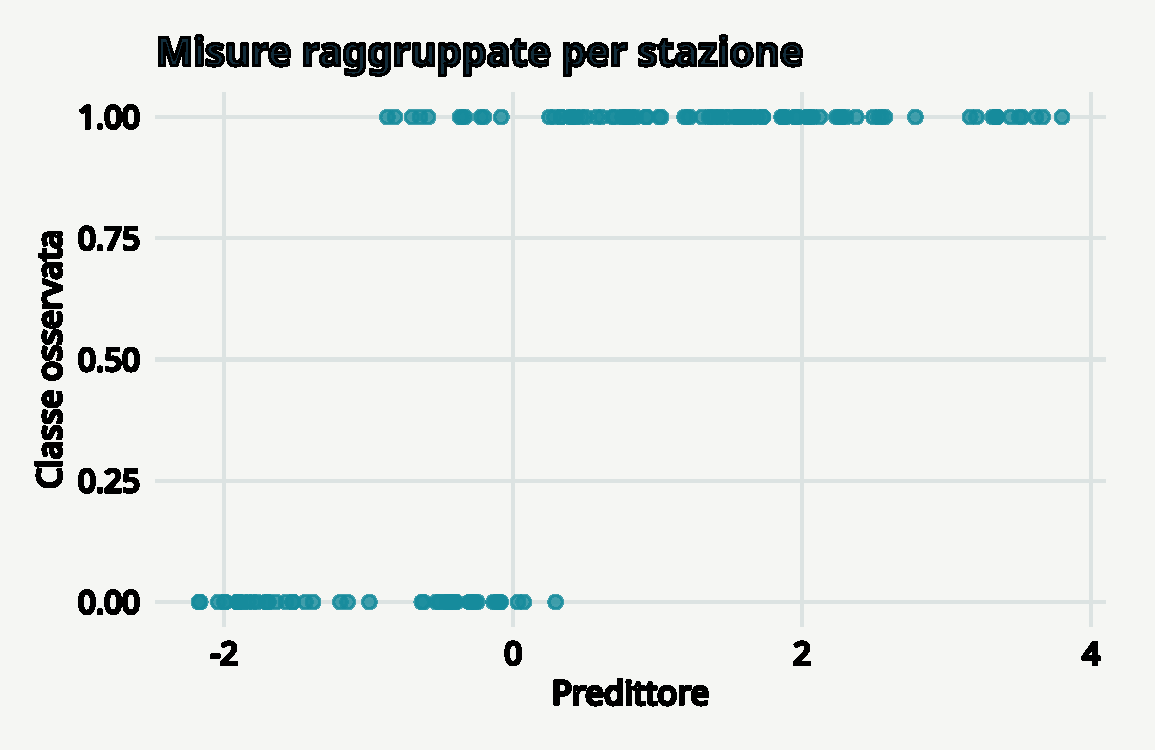
\includegraphics[width=\linewidth,height=6.0cm,keepaspectratio]{Esperimenti/m16-bersaglio-A.pdf}\par}
\PSmall{Ampiezza dell’effetto di stazione: 2. Seme: 17.}
}};
\node[anchor=north west,inner sep=0] at([xshift=10.85cm,yshift=-2.12cm]current page.north west){\Colonna{8.16cm}{\PLabel{Scenario A · simulazione}
\PBody{La validazione di un classificatore deve rappresentare il tipo di osservazione che incontrerà nell’uso futuro. L’esperimento genera misure raggruppate per stazione, con un effetto condiviso che contribuisce sia al predittore sia alla probabilità della classe. Un classificatore a un vicino viene valutato mediante una separazione casuale delle misure e mediante stazioni interamente escluse dall’addestramento.}
\par\smallskip{\centering\adjustbox{max width=.98\linewidth}{$\displaystyle \widehat R=\frac1{n_{test}}\sum_i\mathbf1(\widehat y_i\ne y_i)$}\par\smallskip}
\PSmall{$\hat y_i$ è la classe prevista, $y_i$ quella osservata e $n_{\mathrm{test}}$ il numero di misure escluse dall’addestramento. $\hat R$ è la frequenza degli errori; le metriche dell’interfaccia riportano l’accuratezza, pari a $1-\hat R$.}
}};
\node[anchor=north east,inner sep=0] at([xshift=17.1cm,yshift=-12.04cm]current page.north west){\fontsize{7.7}{9}\selectfont \href{https://marzione00.github.io/Lab_Geo/\#laboratorio/m16-bersaglio}{\color{Classical}\bfseries Apri il laboratorio · m16-bersaglio}};
\end{tikzpicture}\end{frame}

\begin{frame}[plain]\hypertarget{slide21}{}
\bookmark[level=1,page=21]{Confronto | Bersaglio predittivo e nuove stazioni}
\begin{tikzpicture}[remember picture,overlay]
\PilotChrome{Confronto | Bersaglio predittivo e nuove stazioni}{LABORATORI DELLA SPEDIZIONE}{21}{Il protocollo di verifica deve corrispondere all’unità che sarà incontrata nell’uso futuro.}
\node[anchor=north west,inner sep=0] at([xshift=.96cm,yshift=-2.12cm]current page.north west){\Colonna{9.40cm}{{\centering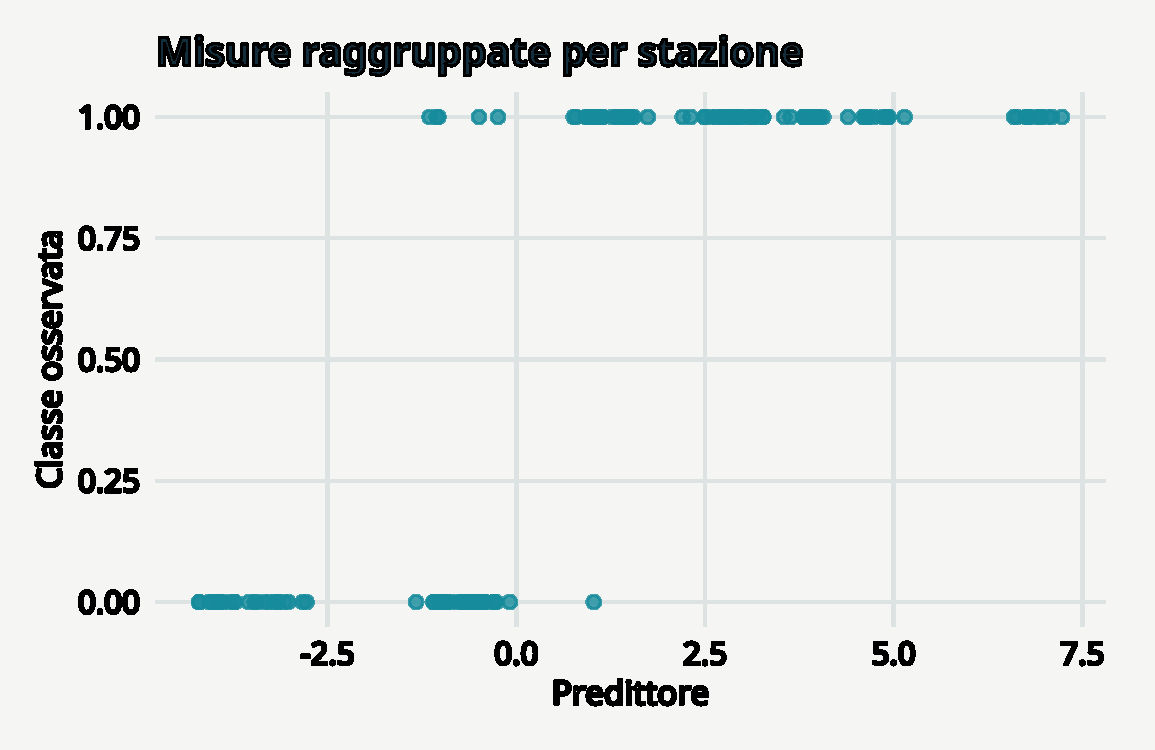
\includegraphics[width=\linewidth,height=5.6cm,keepaspectratio]{Esperimenti/m16-bersaglio-B.pdf}\par}
\PSmall{Ampiezza dell’effetto di stazione: 2 $\to$ 4. Tutti gli altri parametri e il seme sono fissi.}
}};
\node[anchor=north west,inner sep=0] at([xshift=10.85cm,yshift=-2.12cm]current page.north west){\Colonna{8.16cm}{\PLabel{Confronto fra gli scenari}
{\fontsize{10.2}{12.8}\selectfont\begin{tabular}{@{}>{\raggedright\arraybackslash}p{0.48\linewidth}@{\hspace{.13cm}}>{\raggedright\arraybackslash}p{0.224\linewidth}@{\hspace{.13cm}}>{\raggedright\arraybackslash}p{0.224\linewidth}@{}}\toprule Grandezza & A & B\\[2.3pt]
\midrule 
Accuratezza separazione casuale & 0,958 & 0,896\\[2.3pt]
Accuratezza nuove stazioni & 0,75 & 0,729\\[2.3pt]
Stazioni complessive & 12 & 12\\[2.3pt]
\bottomrule\end{tabular}\par}
\vspace{.25cm}\PBody{In entrambi gli scenari l’accuratezza scende quando si escludono stazioni intere. Le prestazioni dipendono dall’unità con cui si costruisce il test.}
}};
\node[anchor=north east,inner sep=0] at([xshift=17.1cm,yshift=-12.04cm]current page.north west){\fontsize{7.7}{9}\selectfont \href{https://marzione00.github.io/Lab_Geo/\#laboratorio/m16-bersaglio}{\color{Classical}\bfseries Apri il laboratorio · m16-bersaglio}};
\end{tikzpicture}\end{frame}

\begin{frame}[plain]\hypertarget{slide22}{}
\bookmark[level=1,page=22]{Selezione dei predittori e contaminazione}
\begin{tikzpicture}[remember picture,overlay]
\PilotChrome{Selezione dei predittori e contaminazione}{LABORATORI DELLA SPEDIZIONE}{22}{Valutare la selezione di variabili su puro rumore.}
\node[anchor=north west,inner sep=0] at([xshift=.96cm,yshift=-2.12cm]current page.north west){\Colonna{9.40cm}{{\centering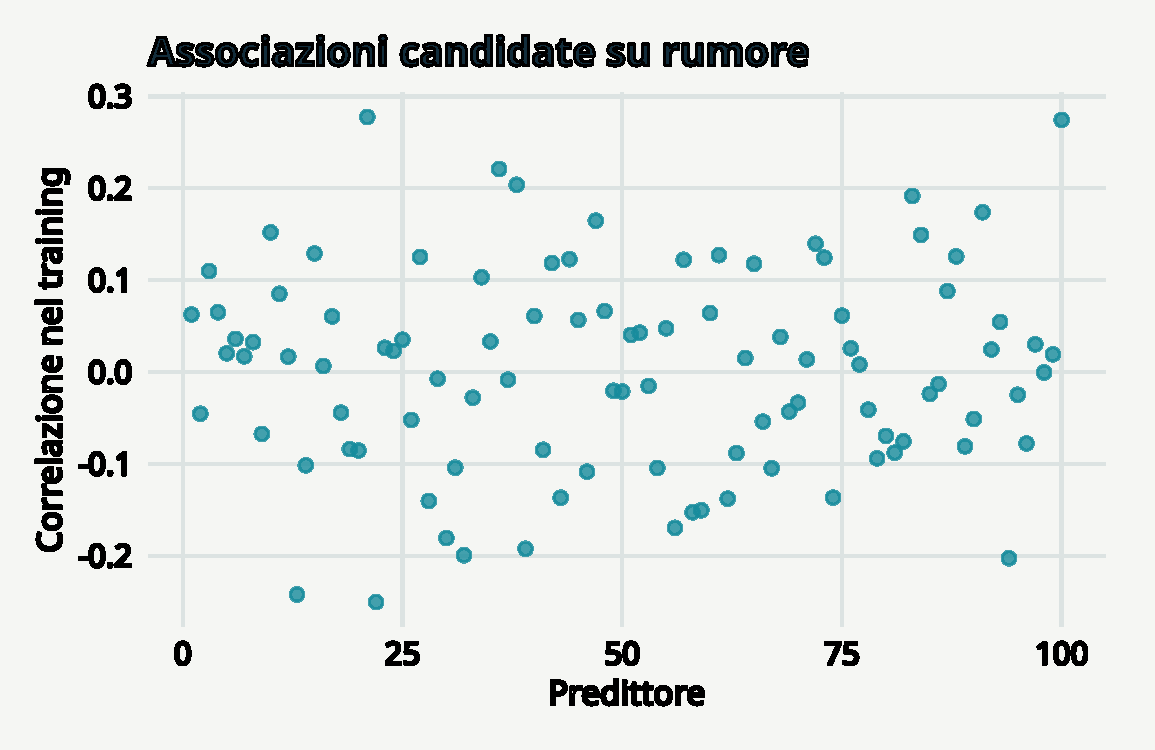
\includegraphics[width=\linewidth,height=6.0cm,keepaspectratio]{Esperimenti/m16-selezione-A.pdf}\par}
\PSmall{Predittori candidati: 100. Seme: 17.}
}};
\node[anchor=north west,inner sep=0] at([xshift=10.85cm,yshift=-2.12cm]current page.north west){\Colonna{8.16cm}{\PLabel{Scenario A · simulazione}
\PBody{La ricerca fra molti predittori può individuare associazioni apparenti anche quando tutte le variabili sono indipendenti dal bersaglio. Nell’esperimento si sceglie il predittore con massima correlazione assoluta, confrontando una selezione eseguita soltanto sul campione di addestramento con una che utilizza anche le risposte del test. Entrambi i modelli vengono poi adattati sul medesimo training.}
\par\smallskip{\centering\adjustbox{max width=.98\linewidth}{$\displaystyle j^*=\arg\max_j|\operatorname{cor}(X_j,Y)|$}\par\smallskip}
\PSmall{$X_j$ è il predittore candidato j, Y la risposta binaria e $j^*$ l’indice selezionato. Il criterio massimizza il valore assoluto della correlazione campionaria, che viene calcolata su insiemi diversi nei due protocolli.}
}};
\node[anchor=north east,inner sep=0] at([xshift=17.1cm,yshift=-12.04cm]current page.north west){\fontsize{7.7}{9}\selectfont \href{https://marzione00.github.io/Lab_Geo/\#laboratorio/m16-selezione}{\color{Classical}\bfseries Apri il laboratorio · m16-selezione}};
\end{tikzpicture}\end{frame}

\begin{frame}[plain]\hypertarget{slide23}{}
\bookmark[level=1,page=23]{Confronto | Selezione dei predittori e contaminazione}
\begin{tikzpicture}[remember picture,overlay]
\PilotChrome{{\fontsize{15.3}{19}\selectfont Confronto | Selezione dei predittori e contaminazione}}{LABORATORI DELLA SPEDIZIONE}{23}{La selezione informata dal test compromette l’indipendenza della valutazione.}
\node[anchor=north west,inner sep=0] at([xshift=.96cm,yshift=-2.12cm]current page.north west){\Colonna{9.40cm}{{\centering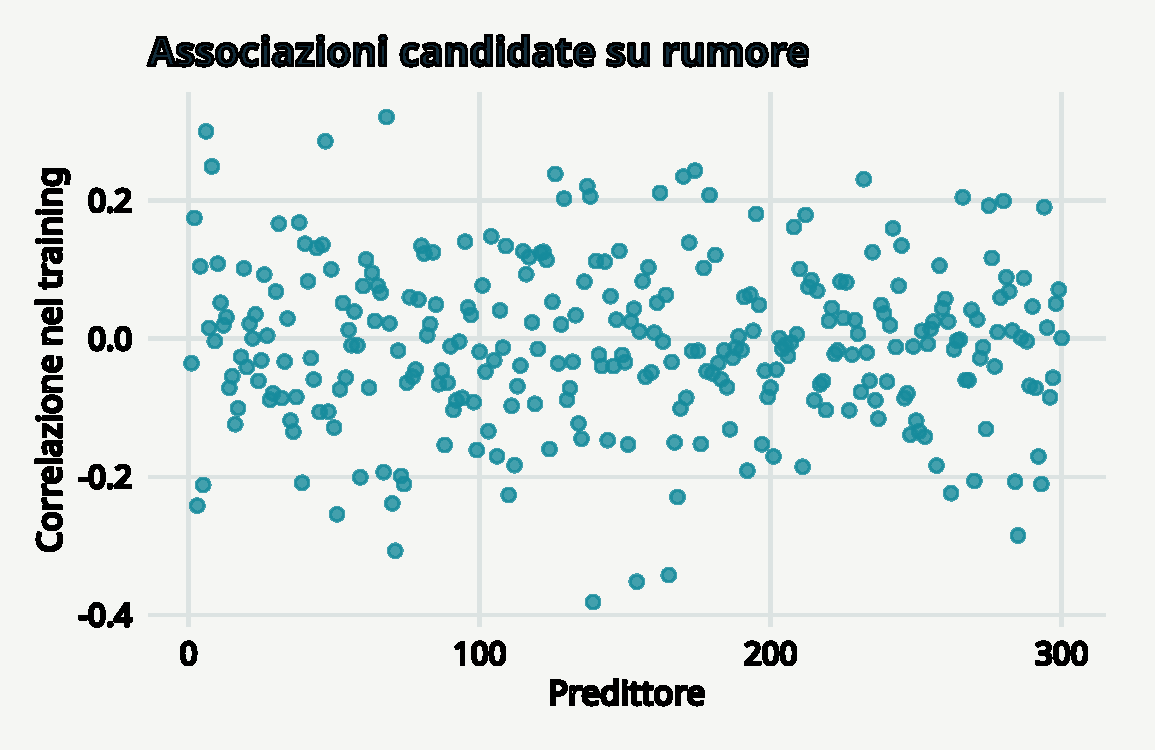
\includegraphics[width=\linewidth,height=5.6cm,keepaspectratio]{Esperimenti/m16-selezione-B.pdf}\par}
\PSmall{Predittori candidati: 100 $\to$ 300. Tutti gli altri parametri e il seme sono fissi.}
}};
\node[anchor=north west,inner sep=0] at([xshift=10.85cm,yshift=-2.12cm]current page.north west){\Colonna{8.16cm}{\PLabel{Confronto fra gli scenari}
{\fontsize{10.2}{12.8}\selectfont\begin{tabular}{@{}>{\raggedright\arraybackslash}p{0.48\linewidth}@{\hspace{.13cm}}>{\raggedright\arraybackslash}p{0.224\linewidth}@{\hspace{.13cm}}>{\raggedright\arraybackslash}p{0.224\linewidth}@{}}\toprule Grandezza & A & B\\[2.3pt]
\midrule 
Accuratezza selezione sul training & 0,45 & 0,375\\[2.3pt]
Accuratezza selezione contaminata & 0,575 & 0,65\\[2.3pt]
Massima correlazione assoluta training & 0,277 & 0,381\\[2.3pt]
\bottomrule\end{tabular}\par}
\vspace{.25cm}\PBody{Con più candidati cresce l’opportunità di trovare associazioni casuali. La selezione contaminata dal test appare più favorevole in questo campione.}
}};
\node[anchor=north east,inner sep=0] at([xshift=17.1cm,yshift=-12.04cm]current page.north west){\fontsize{7.7}{9}\selectfont \href{https://marzione00.github.io/Lab_Geo/\#laboratorio/m16-selezione}{\color{Classical}\bfseries Apri il laboratorio · m16-selezione}};
\end{tikzpicture}\end{frame}

\begin{frame}[plain]\hypertarget{slide24}{}
\bookmark[level=1,page=24]{Soglia, discriminazione e calibrazione}
\begin{tikzpicture}[remember picture,overlay]
\PilotChrome{Soglia, discriminazione e calibrazione}{LABORATORI DELLA SPEDIZIONE}{24}{Separare probabilità previste e decisione binaria.}
\node[anchor=north west,inner sep=0] at([xshift=.96cm,yshift=-2.12cm]current page.north west){\Colonna{9.40cm}{{\centering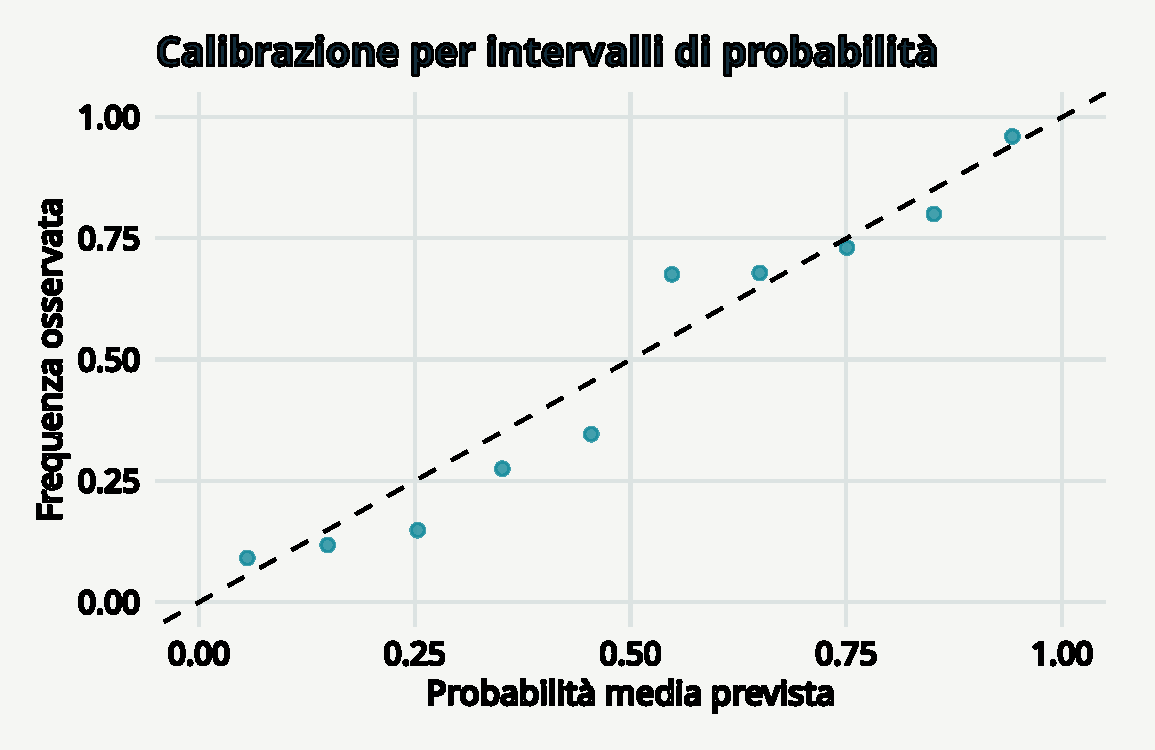
\includegraphics[width=\linewidth,height=6.0cm,keepaspectratio]{Esperimenti/m16-metriche-A.pdf}\par}
\PSmall{Soglia decisionale: 0,5. Seme: 17.}
}};
\node[anchor=north west,inner sep=0] at([xshift=10.85cm,yshift=-2.12cm]current page.north west){\Colonna{8.16cm}{\PLabel{Scenario A · simulazione}
\PBody{Una previsione probabilistica e una decisione binaria rispondono a valutazioni differenti. L’esperimento genera risposte da probabilità logistiche note e modifica le probabilità dichiarate moltiplicandone il logit. Un controllo separato stabilisce la soglia con cui trasformare tali probabilità in classi, rendendo confrontabili calibrazione e conseguenze della decisione.}
\par\smallskip{\centering\adjustbox{max width=.98\linewidth}{$\displaystyle \operatorname{Brier}=n^{-1}\sum_i(p_i-y_i)^2$}\par\smallskip}
\PSmall{$p_i$ è la probabilità dichiarata per l’osservazione i, $y_i$ la risposta binaria e n la numerosità. Il Brier score è la media dei quadrati degli scarti fra probabilità e risposte; valori inferiori indicano previsioni probabilistiche migliori nel campione valutato.}
}};
\node[anchor=north east,inner sep=0] at([xshift=17.1cm,yshift=-12.04cm]current page.north west){\fontsize{7.7}{9}\selectfont \href{https://marzione00.github.io/Lab_Geo/\#laboratorio/m16-metriche}{\color{Classical}\bfseries Apri il laboratorio · m16-metriche}};
\end{tikzpicture}\end{frame}

\begin{frame}[plain]\hypertarget{slide25}{}
\bookmark[level=1,page=25]{Confronto | Soglia, discriminazione e calibrazione}
\begin{tikzpicture}[remember picture,overlay]
\PilotChrome{Confronto | Soglia, discriminazione e calibrazione}{LABORATORI DELLA SPEDIZIONE}{25}{Una soglia modifica le decisioni, mentre la calibrazione riguarda il significato delle probabilità.}
\node[anchor=north west,inner sep=0] at([xshift=.96cm,yshift=-2.12cm]current page.north west){\Colonna{9.40cm}{{\centering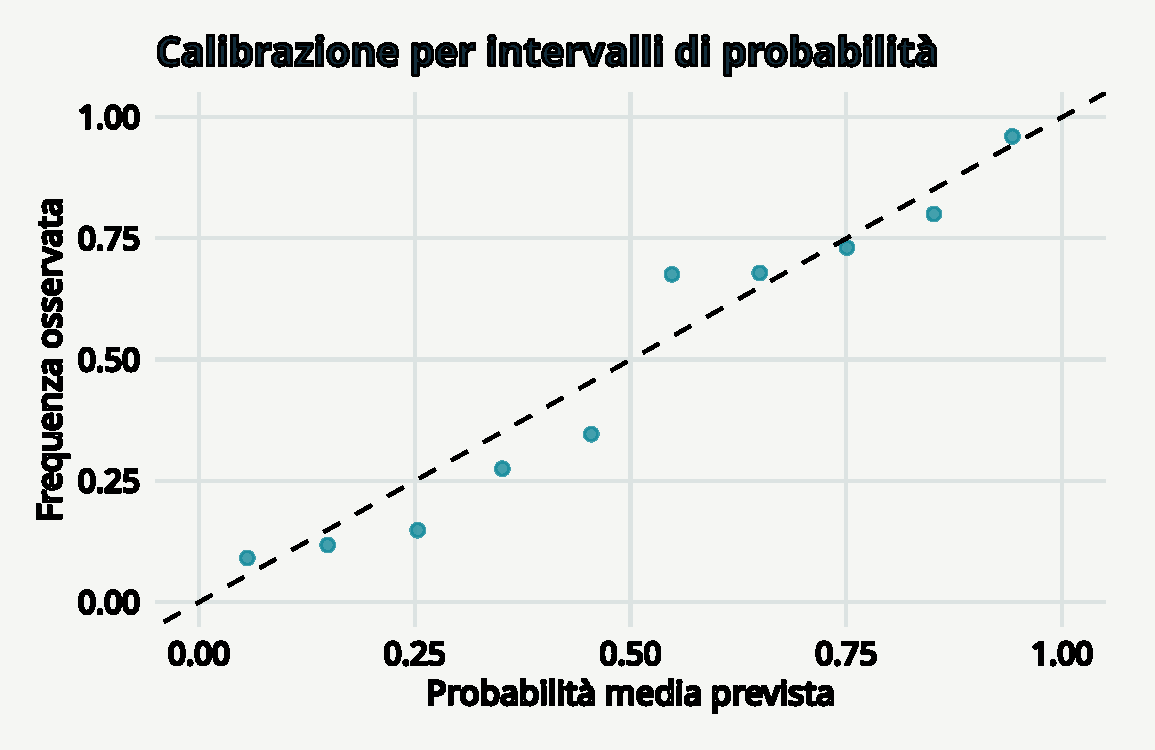
\includegraphics[width=\linewidth,height=5.6cm,keepaspectratio]{Esperimenti/m16-metriche-B.pdf}\par}
\PSmall{Soglia decisionale: 0,5 $\to$ 0,75. Tutti gli altri parametri e il seme sono fissi.}
}};
\node[anchor=north west,inner sep=0] at([xshift=10.85cm,yshift=-2.12cm]current page.north west){\Colonna{8.16cm}{\PLabel{Confronto fra gli scenari}
{\fontsize{10.2}{12.8}\selectfont\begin{tabular}{@{}>{\raggedright\arraybackslash}p{0.48\linewidth}@{\hspace{.13cm}}>{\raggedright\arraybackslash}p{0.224\linewidth}@{\hspace{.13cm}}>{\raggedright\arraybackslash}p{0.224\linewidth}@{}}\toprule Grandezza & A & B\\[2.3pt]
\midrule 
Veri positivi & 115 & 61\\[2.3pt]
Falsi positivi & 36 & 10\\[2.3pt]
Veri negativi & 119 & 145\\[2.3pt]
Falsi negativi & 30 & 84\\[2.3pt]
Sensibilità & 0,793 & 0,421\\[2.3pt]
Specificità & 0,768 & 0,935\\[2.3pt]
Brier score & 0,168 & 0,168\\[2.3pt]
\bottomrule\end{tabular}\par}
\vspace{.25cm}\PBody{Alzando la soglia da 0,50 a 0,75 diminuiscono sia i veri sia i falsi positivi. Il Brier score è invariato perché usa le probabilità prima della soglia.}
}};
\node[anchor=north east,inner sep=0] at([xshift=17.1cm,yshift=-12.04cm]current page.north west){\fontsize{7.7}{9}\selectfont \href{https://marzione00.github.io/Lab_Geo/\#laboratorio/m16-metriche}{\color{Classical}\bfseries Apri il laboratorio · m16-metriche}};
\end{tikzpicture}\end{frame}

\begin{frame}[plain]\hypertarget{slide26}{}
\bookmark[level=1,page=26]{Dal risultato alla relazione}
\begin{tikzpicture}[remember picture,overlay]
\PilotChrome{Dal risultato alla relazione}{SINTESI}{26}{Riporta accuratezza, denominatori, riferimento e dominio di validità del classificatore.}
\node[anchor=north west,inner sep=0] at([xshift=.96cm,yshift=-2.12cm]current page.north west){\Colonna{9.40cm}{\PLabel{Domanda di partenza}
\PBody{Il classificatore dei centroidi riconosce la litologia di stazioni escluse dall’adattamento?}
\PLabel{Risultato da discutere}
\PBody{Sui trenta provini delle tre stazioni escluse il classificatore dei centroidi assegna tutte le litologie osservate, contro il riferimento di 0,333 della classe più frequente. I margini fra la seconda e la prima distanza quadratica vanno da circa 5,19 a 17,80.}
}};
\node[anchor=north west,inner sep=0] at([xshift=10.85cm,yshift=-2.12cm]current page.north west){\Colonna{8.16cm}{\PLabel{Limiti della conclusione}
\PBody{Le classi sono sintetiche e ben separate, e il test era già noto nel percorso didattico. Una roccia di una litologia non inclusa riceverebbe comunque una delle tre etichette, per cui un campione nuovo richiede anche una verifica di pertinenza al dominio.}
\vspace{.4cm}\href{https://marzione00.github.io/Lab_Geo/\#progetti}{\color{Classical}\bfseries Torna all’elenco delle spedizioni}
}};
\end{tikzpicture}\end{frame}

\begin{frame}[plain]\hypertarget{slide27}{}
\bookmark[level=1,page=27]{Fonti, dati e codice per riprodurre le figure}
\begin{tikzpicture}[remember picture,overlay]
\PilotChrome{Fonti, dati e codice per riprodurre le figure}{RIFERIMENTI}{27}{I risultati numerici si riferiscono ai dati e alle ipotesi dichiarate nel caso.}
\node[anchor=north west,inner sep=0] at([xshift=.96cm,yshift=-2.12cm]current page.north west){\Colonna{9.40cm}{\PLabel{Dati e attribuzioni}
\PBody{Dati sintetici del corso (ml\_v3.csv): centottanta provini di diciotto stazioni con SiO$_2$, CaO, MgO, FeO e densità, in raccordo con il modulo M16.}
}};
\node[anchor=north west,inner sep=0] at([xshift=10.85cm,yshift=-2.12cm]current page.north west){\Colonna{8.16cm}{\PLabel{Nell’archivio dei sorgenti}
\PBody{Codice contiene i frammenti delle pagine; R contiene lo script P11\_figure.R, che ricostruisce figure e valori dai dati. Esperimenti comprende i programmi dei due scenari, Diagrammi i disegni TikZ modificabili, Scena il modello Blender della copertina.}
\vspace{.4cm}\href{https://marzione00.github.io/Lab_Geo/\#modulo-P11}{\color{Classical}\bfseries Apri la spedizione P11 su GeoStat Lab}
}};
\end{tikzpicture}\end{frame}
\end{document}
